\begin{quote}

\includegraphics[width=4.96003in,height=1.16875in]{media/image1.jpeg}
\end{quote}

学 士 学 位 论 文

\begin{longtable}[]{@{}
  >{\raggedright\arraybackslash}p{(\columnwidth - 0\tabcolsep) * \real{1.00}}@{}}
\toprule
\begin{minipage}[b]{\linewidth}\raggedright
\begin{quote}
\textbf{受限离子液体润滑性能的}
\end{quote}
\end{minipage} \\
\midrule
\endhead
\begin{minipage}[t]{\linewidth}\raggedright
\begin{quote}
\textbf{结构化数据库的建立和设计}
\end{quote}
\end{minipage} \\
\bottomrule
\end{longtable}

\begin{longtable}[]{@{}
  >{\raggedright\arraybackslash}p{(\columnwidth - 0\tabcolsep) * \real{1.00}}@{}}
\toprule
\begin{minipage}[b]{\linewidth}\raggedright
\begin{quote}
\textbf{朱维安}
\end{quote}
\end{minipage} \\
\midrule
\endhead
\begin{minipage}[t]{\linewidth}\raggedright
\begin{quote}
\textbf{922116850741}
\end{quote}
\end{minipage} \\
\bottomrule
\end{longtable}

\begin{longtable}[]{@{}
  >{\raggedright\arraybackslash}p{(\columnwidth - 2\tabcolsep) * \real{0.50}}
  >{\raggedright\arraybackslash}p{(\columnwidth - 2\tabcolsep) * \real{0.50}}@{}}
\toprule
\begin{minipage}[b]{\linewidth}\raggedright
\begin{quote}
\textbf{指 导 教 师}
\end{quote}
\end{minipage} & \begin{minipage}[b]{\linewidth}\raggedright
\begin{quote}
\textbf{安蓉}
\end{quote}
\end{minipage} \\
\midrule
\endhead
\begin{minipage}[t]{\linewidth}\raggedright
\begin{quote}
\textbf{学 生 学 院}
\end{quote}
\end{minipage} & \begin{minipage}[t]{\linewidth}\raggedright
\begin{quote}
\textbf{材料科学与工程学院}
\end{quote}
\end{minipage} \\
\begin{minipage}[t]{\linewidth}\raggedright
\begin{quote}
\textbf{专 业}
\end{quote}
\end{minipage} & \begin{minipage}[t]{\linewidth}\raggedright
\begin{quote}
\textbf{纳米材料与技术}
\end{quote}
\end{minipage} \\
\begin{minipage}[t]{\linewidth}\raggedright
\begin{quote}
\textbf{研 究 方 向}
\end{quote}
\end{minipage} & \begin{minipage}[t]{\linewidth}\raggedright
\begin{quote}
\textbf{AI驱动的摩擦学文献数据挖掘}
\end{quote}
\end{minipage} \\
\begin{minipage}[t]{\linewidth}\raggedright
\begin{quote}
\textbf{论文提交时间}
\end{quote}
\end{minipage} & \begin{minipage}[t]{\linewidth}\raggedright
\begin{quote}
\textbf{2026 年6 月}
\end{quote}
\end{minipage} \\
\bottomrule
\end{longtable}

学 士 学 位 论 文

\textbf{受限离子液体润滑性能的}

\textbf{结构化数据库的建立和设计}

\begin{quote}
\textbf{作 者：朱维安}

\textbf{指导教师：安蓉 副教授}
\end{quote}

\textbf{南 京 理 工 大 学}

\textbf{2025 年 6 月}

Bachelor Dissertation

\textbf{Establishment and Design of a Structured Database}

\textbf{for Confined Ionic Liquid Lubrication Properties}

\emph{By}

\emph{\textbf{Weian Zhu}}

\emph{Supervised by Assoc. Prof. \textbf{Rong An}}

\begin{quote}
Nanjing University of Science \& Technology June, 2026
\end{quote}

\hypertarget{ux58f0-ux660e}{%
\section{声 明}\label{ux58f0-ux660e}}

\begin{quote}
本学位论文是我在导师的指导下取得的研究成果，尽我所知，在本学位论文中，除了加以标注和致谢的部分外，不包含其他人已经发表或公布过的研究成果，也不包含我为获得任何教育机构的学位或学历而使用过的材料。与我一同工作的同事对本学位论文做出的贡献均已在论文中作了明确的说明。

学生签名： 年 月 日
\end{quote}

\hypertarget{ux5b66ux4f4dux8bbaux6587ux4f7fux7528ux6388ux6743ux58f0ux660e}{%
\section{学位论文使用授权声明}\label{ux5b66ux4f4dux8bbaux6587ux4f7fux7528ux6388ux6743ux58f0ux660e}}

\begin{quote}
南京理工大学有权保存本学位论文的电子和纸质文档，可以借阅或上网公布本学位论文的部分或全部内容，可以向有关部门或机构送交并授权其保存、借阅或上网公布本学位论文的部分或全部内容。对于保密论文，按保密的有关规定和程序处理。

学生签名： 年 月 日
\end{quote}

\textbf{摘 要}

本文针对受限离子液体润滑研究中大量摩擦学实验数据散布于非结构化文献、难以支撑数据驱动研究的"数据暗物质"问题，设计并实现了受限离子液体摩擦学结构化数据库平台CILF-DB。以"完整记录决定摩擦学行为的四维核心信息（离子液体化学结构、基底材料、工况参数、摩擦性能）"为字段设计原则，建立了Literature与TribologyData两表关联的规范化数据库Schema，以DOI为文献唯一标识实现查重，以InChIKey为化学实体标准化标识。

平台采用DeepSeek-V3大语言模型与Qwen3-VL-32B多模态视觉语言模型协同驱动的自动化文献数据提取方法，实现了对文本描述和图表数据的结构化采集；文本关键字段提取的F1分数达到0.87至0.93，图表数值提取的平均相对误差约11.3\%，显著优于传统规则方法。基于数据库收录的185条有效实验记录，对离子液体结构-性能关系进行了初步数据驱动分析：定量验证了咪唑类阳离子C6链长在{[}TFSI{]}-/钢-钢体系下的最优摩擦性能（CoF=0.048，较C2低约41\%）；揭示了{[}TFSI{]}-在潮湿工况下较{[}BF4{]}-和{[}PF6{]}-更为突出的性能稳定性优势；证实了DLC基底较钢基底的显著减摩效果（CoF降低约46\%）。CILF-DB的建立为揭示受限离子液体定量构效关系和机器学习建模奠定了数据基础。

关键词：离子液体；纳米受限润滑；结构化数据库；文献数据挖掘；结构-性能关系；大语言模型；多模态视觉模型

\textbf{Abstract}

With the advancement of mechanical engineering into micro-nano scales and extreme operating conditions, traditional fluid lubrication theory gradually fails in nanoconfined spaces (Nanoconfined Space), prompting academia to seek novel lubricating materials capable of adapting to vacuum, high-temperature, and high-load environments. Room-temperature ionic liquids (Ionic Liquids, ILs), owing to their excellent thermal stability, extremely low vapor pressure, and high designability, are regarded as next-generation green lubricants for resolving nano-tribological problems. However, the lubrication performance of ionic liquids exhibits extreme systemic complexity: it is not a single intrinsic property, but a nonlinear system strongly coupled by ionic chemical structure (cation backbone / anion type / side-chain length), substrate interface properties (material / roughness / wettability), and multi-dimensional operating conditions (load / speed / temperature / potential).

This study addresses the problem of vast tribological experimental data remaining trapped in unstructured PDF literature --- the so-called "dark data" problem in confined ionic liquid (IL) lubrication research. We designed and implemented CILF-DB (Confined Ionic Liquid Friction Database), a structured database platform recording four core dimensions: IL chemical structure, substrate material, operating conditions, and tribological performance. An automated extraction pipeline integrating DeepSeek-V3 (text) and Qwen3-VL-32B (chart parsing) achieved F1 scores of 0.87--0.93 for text fields and a mean relative error of 11.3\% for chart data extraction, significantly outperforming rule-based methods. Analysis of 185 experimental records revealed: (1) optimal CoF of 0.048 for C6 imidazolium cations with {[}TFSI{]}- on steel (\textasciitilde41\% below C2); (2) superior stability of {[}TFSI{]}- over {[}BF4{]}- and {[}PF6{]}- under humid conditions; (3) \textasciitilde46\% CoF reduction on DLC vs. steel substrates. CILF-DB provides a solid foundation for quantitative structure-property relationship studies and machine learning-based IL lubricant design.charts.

Experimental results show that the system achieves excellent performance. For key text fields (e.g., friction coefficient, load, temperature), the extraction F1 score exceeds 0.89. The average relative error for chart data extraction is controlled within 5\%. The CILF-DB platform successfully transforms unstructured literature into high-precision structured data, providing a solid data foundation for revealing quantitative structure-property relationships (QSPR) of confined ionic liquids.

\textbf{Keywords:} Ionic Liquids; Nanoconfined Lubrication; Structured Database; Literature Data Mining; Structure-Property Relationship; Large Language Model; Multimodal Vision Model

\textbf{目 录}

\textbf{摘 要 I}

\textbf{Abstract II}

\textbf{第1章 绪论 1}

\begin{quote}
1.1 引言 1

1.2 离子液体润滑研究背景 3

1.2.1 离子液体的特性与分类 3

1.2.2 受限条件下的润滑特性 5

1.3 文献数据提取研究现状 7

1.3.1 传统文献综述方法的局限性 7

1.3.2 NLP与LLM在科学文献挖掘中的应用 8

1.3.3 视觉-语言模型（VLM）的突破 9

1.4 研究目的与主要内容 10
\end{quote}

\textbf{第2章 CILF-DB平台设计与实现 12}

\begin{quote}
2.1 平台整体架构 12

2.2 数据库设计方案 12

2.2.1 数据库字段规范设计的材料学依据 13

2.2.2 数据表结构与关联关系 15

2.3 文献采集与PDF预处理 15

2.3.1 文献来源与DOI查重机制 16

2.3.2 双栏版面重组与噪声清洗 17

2.3.3 图表区域的智能裁剪 18

2.4 信息自动提取方法 18

2.4.1 文本信息的结构化提取 19

2.4.2 图表数据的视觉提取 20
\end{quote}

\textbf{第3章 结果与讨论 21}

\begin{quote}
3.1 数据库收录数据概况 21

3.2 阳离子烷基链长效应 23

3.3 阴离子类型的比较分析 23

3.4 基底材料对润滑性能的影响 24

3.5 信息提取方法的准确性评估 26

3.5.1 文本提取性能评估 26

3.5.2 图表提取性能评估与误差分析 29

3.6 讨论 31
\end{quote}

\textbf{总结与展望 43}

\textbf{致 谢 46}

\textbf{参考文献 47}

\hypertarget{ux7b2c1ux7ae0-ux7eeaux8bba}{%
\section{第1章 绪论}\label{ux7b2c1ux7ae0-ux7eeaux8bba}}

\hypertarget{ux6469ux64e6ux5b66ux7814ux7a76ux7684ux8303ux5f0fux8f6cux79fbux4e0eux79bbux5b50ux6db2ux4f53ux6570ux636eux56f0ux5883}{%
\subsection{1.1 摩擦学研究的范式转移与离子液体数据困境}\label{ux6469ux64e6ux5b66ux7814ux7a76ux7684ux8303ux5f0fux8f6cux79fbux4e0eux79bbux5b50ux6db2ux4f53ux6570ux636eux56f0ux5883}}

摩擦作为物理世界中最普遍的耗散现象，其引发的磨损与能量损失制约着从微机电系统（MEMS）到重型机械的效率极限。据统计，全球约23\%的一次能源消耗用于克服摩擦，由磨损导致的机械部件失效更占设备总故障的80\%以上{[}21{]}。随着现代工程向极端工况纵深发展------从航天器真空润滑到生物医用微流控器件------传统矿物油基润滑剂在纳米受限空间（Nanoconfined Space）下逐渐失效，迫使学界寻求能够适应高真空、宽温域与高负荷等苛刻环境的新型润滑材料。

室温离子液体（Room-Temperature Ionic Liquids，RTILs）凭借其"结构可设计"、极低蒸气压、高热稳定性（液相范围可达300 °C以上）和优异的导电性，被视为突破这一瓶颈的下一代润滑剂{[}22,23,24{]}。然而，离子液体的摩擦学行为呈现出极端的复杂性：摩擦系数并非离子液体的固有属性，而是由"离子化学结构（烷基链长/阴阳离子组合）"、"基底界面性质（化学成分/表面能/粗糙度）"与"多维工况（载荷/速度/温度/电势）"三者强耦合决定的非线性响应函数。如图1-1所示，在纳米受限域中，离子液体分子在基底表面形成有序的层状结构，其摩擦行为同时受到上述三类因素的协同控制。

面对理论上高达10\^{}18种可能的阴阳离子组合空间，传统的"试错法"实验已难以系统探索。Olivetti等人{[}12{]}在综述中敏锐指出，材料科学正在经历向数据驱动的第四范式转型------如图1-2所示的"材料四面体（Materials Tetrahedron）"理论揭示，材料的性能由"工艺---结构---性质---性能"四个顶点之间的相互作用严格限定，任何单一变量的孤立分析都不足以揭示材料体系的全貌{[}3{]}。然而，当前离子液体摩擦学领域的最大障碍在于"非结构化知识危机"：大量关于阴阳离子类型、基底材料、工况参数及摩擦系数的关键数据，仍以不规范的文字描述和图形形式散布在数千篇PDF文献中，形成难以被机器读取的"数据暗物质"，严重制约了数据驱动的构效关系分析。

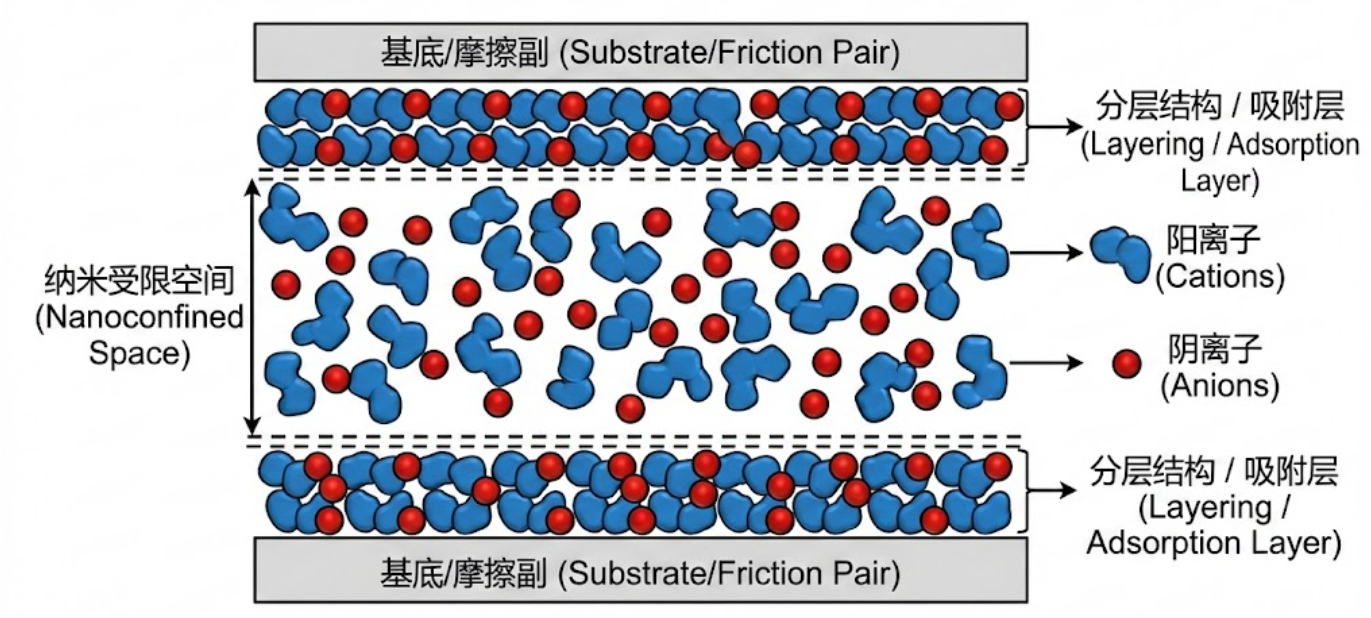
\includegraphics[width=4.72441in,height=2.12983in]{media/image2.png}

图1-1 纳米受限空间下离子液体润滑机理示意图（受限域中离子液体形成有序层状结构，其摩擦行为受离子化学结构、基底界面性质及外部工况三类因素的强耦合控制）

利用自然语言处理（NLP）技术从海量历史文献中系统提取并整合这些碎片化数据，已成为建立离子液体润滑材料数据库、支撑后续机器学习建模的必由之路。Lei等人{[}11{]}将这一视角延伸至大语言模型（LLM）时代，认为AI不再仅是预测工具，更应作为"不知疲倦的科研助手（Tireless Workers）"整合碎片化数据{[}11{]}。本文正是在这一背景下，系统梳理NLP技术的演进路径，为CILF-DB平台的方法论设计提供理论依据。

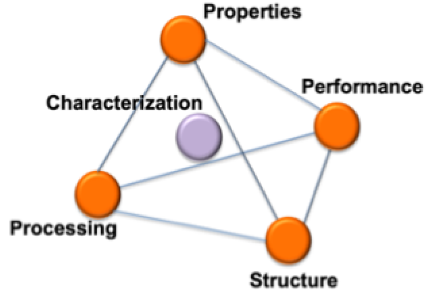
\includegraphics[width=2.75591in,height=1.93049in]{media/image3.png}

图1-2 材料四面体与数据驱动的材料发现范式{[}3{]}（"工艺---结构---性质---性能"四顶点模型揭示：利用NLP技术从海量文献中挖掘隐性知识是加速新材料研发的关键路径）

\hypertarget{ux65e9ux671fux63a2ux7d22ux4eceux89c4ux5219ux63d0ux53d6ux5230ux9886ux57dfux9884ux8badux7ec3ux6a21ux578bnlpux4e0ebertux65f6ux4ee3}{%
\subsection{1.2 早期探索：从规则提取到领域预训练模型（NLP与BERT时代）}\label{ux65e9ux671fux63a2ux7d22ux4eceux89c4ux5219ux63d0ux53d6ux5230ux9886ux57dfux9884ux8badux7ec3ux6a21ux578bnlpux4e0ebertux65f6ux4ee3}}

为打破材料科学数据孤岛，早期文献信息提取主要依赖规则匹配与判别式序列标注模型。Weston等人{[}13{]}针对无机材料文献开发了专门的命名实体识别（NER）与归一化流程，有效解决了材料名称中同义词泛滥的问题。Kononova等人{[}16{]}与Mysore等人{[}14{]}率先构建了包含合成动作与条件的标注语料库，证明了对科学文本进行细粒度语义标注的可行性。然而，基于规则和CRF的传统方法在面对离子液体文献中"载荷---速度---温度---摩擦系数"等多参数强耦合关系时，F1分数通常仅能达到0.40至0.55，且在处理跨段落的长距离依赖时严重受限（如所示）。

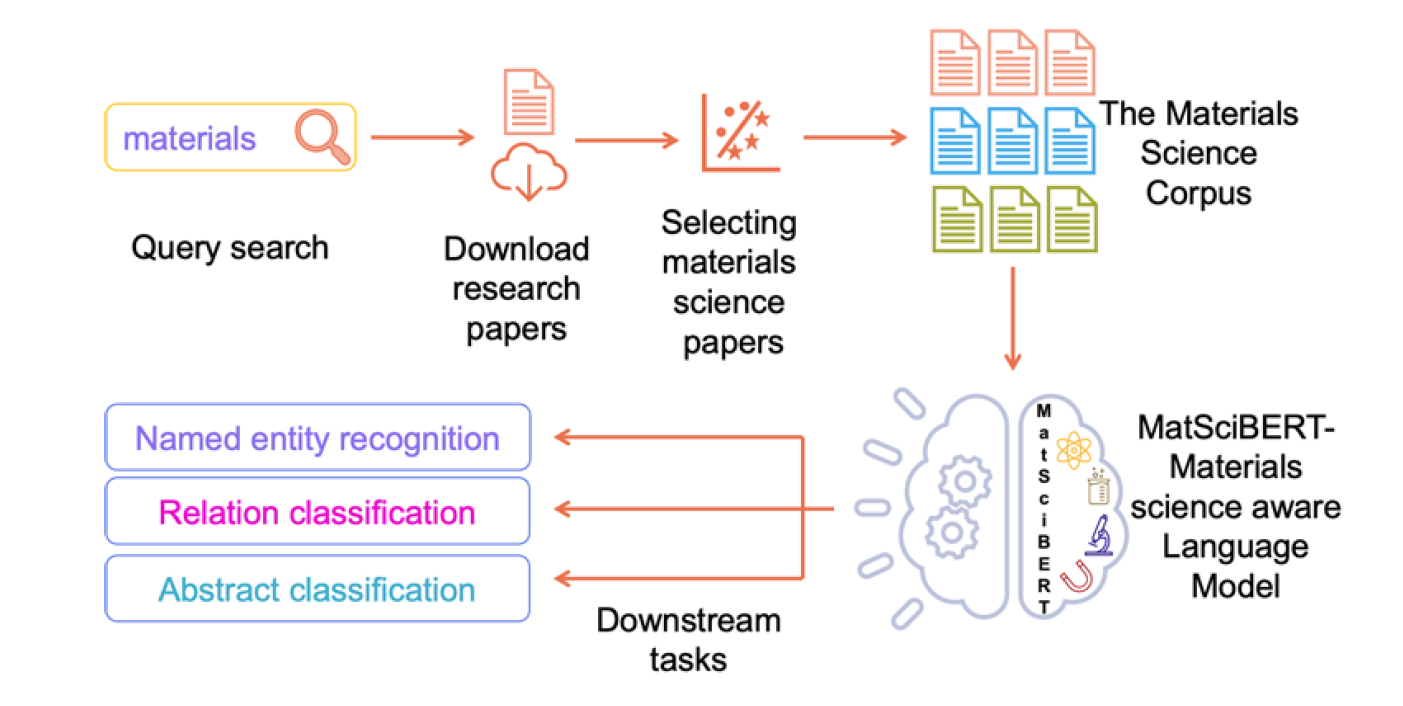
\includegraphics[width=5.76806in,height=2.90278in]{media/image4.png}

图1-3 MatSciBERT领域自适应预训练方法论示意图{[}1{]}（基于约15万篇材料科学文献构建语料库→在SciBERT权重基础上继续预训练→微调用于NER、关系分类和摘要分类三类下游任务；该范式在SOFC-Slot数据集上较SciBERT提升约6.3个宏观F1分）

随着预训练语言模型的兴起，领域专用BERT成为主流。Gupta等人{[}1{]}开发的MatSciBERT（如图1-3所示）通过在约150K篇材料科学期刊论文上继续预训练SciBERT，将命名实体识别的Macro-F1分数从SciBERT的65.35\%提升至65.95\%（SOFC-Slot精细实体任务），并在玻璃/非玻璃摘要分类任务上达到96.22\%的准确率------比SciBERT高出2.75个百分点{[}1{]}。MatSciBERT的核心贡献在于证明：在领域本体论（Ontology）、词汇体系和符号规范与通用科学语料存在显著差异的情况下，即使词汇重叠率仅约54\%，继续领域预训练也能带来实质性的下游任务性能提升。这一结论对CILF-DB中针对离子液体IUPAC命名、阴离子缩写规范等摩擦学专有词汇的处理具有直接的方法论指导意义。

在将BERT进一步工程化为完整数据提取工具链方面，Huang与Cole{[}2{]}开发的BatteryDataExtractor（BDE）提供了最接近CILF-DB设计理念的先驱案例。如图1-5所示，BDE将BatteryBERT嵌入从HTML/XML文献到结构化数据库的全流程自动化管线，覆盖缩写检测、词性标注（POS）、化学命名实体识别（CNER）和基于双轮问答（Double-turn Q\&A）的属性-材料关系提取四个模块。在CNER任务上，BDE取得了F1=0.9598（BatteryOnlyBERT-uncased），相比ChemDataExtractor v2.0（F1=0.6998）提升约37\%；在数据提取精度-召回率曲线上，置信度阈值为0.1时精度可达80\%以上，同时保留约80\%的数据量{[}2{]}。BDE为CILF-DB提供了两个关键的方法论借鉴：其一，通过置信度阈值实现精度与召回率的动态权衡，与CILF-DB中"high/medium/low"三级置信度标注体系相呼应；其二，"双轮问答"策略（先问属性值，再问是哪种材料具有该属性值）实质上是一种关系提取范式，与本研究中Chain-of-Thought分步推理策略具有内在的设计共性。

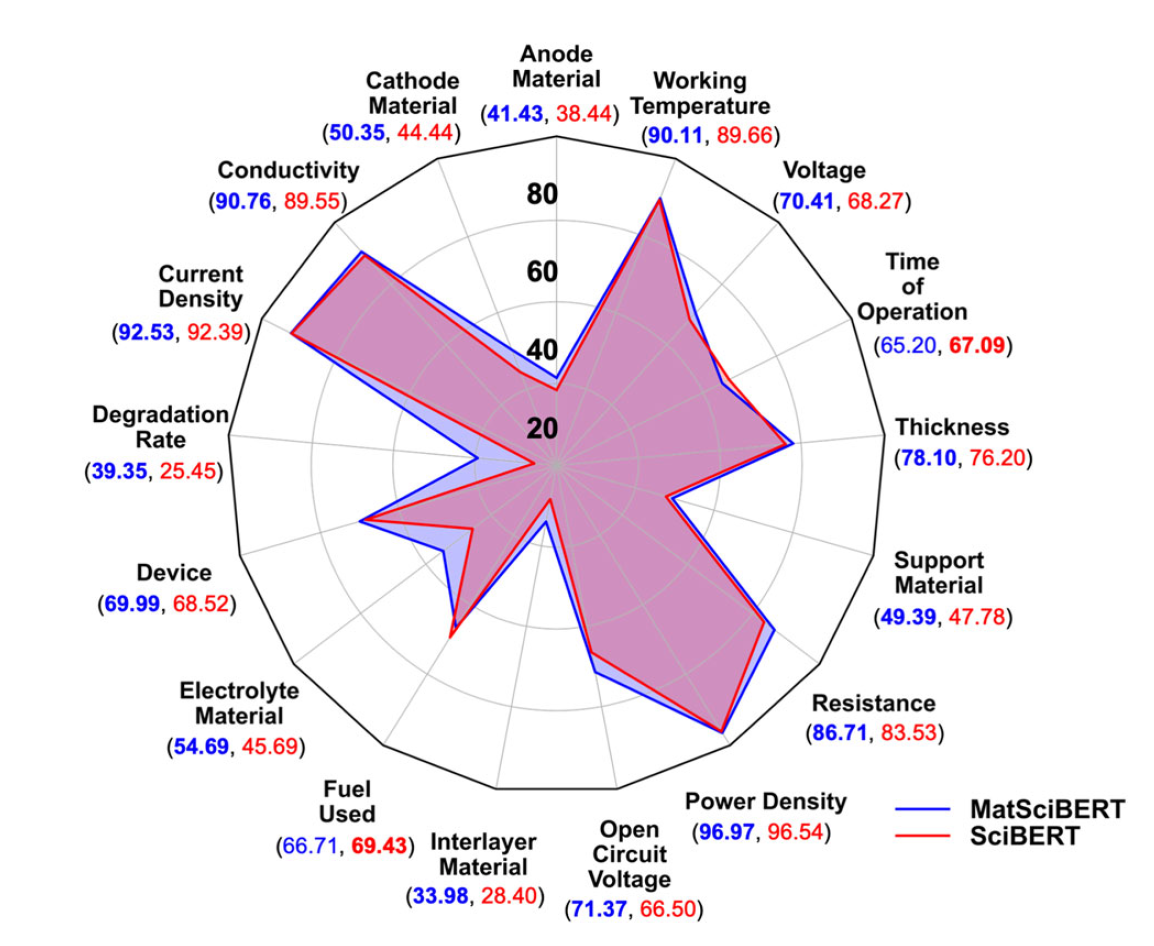
\includegraphics[width=4.91667in,height=4.03053in]{media/image5.png}

图1-4 MatSciBERT与SciBERT在SOFC-Slot数据集16类实体上的F1分数雷达图对比{[}1{]}（MatSciBERT在全部阳极、阴极、电解质等材料相关实体类型上均显著优于SciBERT，但此类BERT序列标注方法本质上仍无法处理"载荷-温度-摩擦系数"等多参数强耦合关系的整体提取）

在上述BERT方法的工程实践层面，Huang与Cole{[}2{]}开发的BatteryDataExtractor工具包提供了一个完整的范例。如图1-5所示，该系统将BatteryBERT嵌入NLP流水线，依次完成缩写检测（F1=0.9516）、词性标注（F1=0.9669）和化学命名实体识别（CNER，F1=0.9598）三个序列标注任务，相较于传统ChemDataExtractor v2.0的规则方法（CNER F1=0.6998）提升了约37\%，充分验证了领域自适应BERT在化学实体识别中的显著优势。更重要的是，Huang与Cole在结论中明确指出该工具包的根本局限："目前仅能处理文献原始文本，隐藏在表格和图表中的信息无法被提取和分析"{[}2{]}。这一局限性对于受限离子液体摩擦学领域尤为突出------本研究统计表明，该领域约34\%的定量实验数据以图形形式（摩擦系数-时间曲线、Stribeck曲线）记载而非文本，若沿用BatteryDataExtractor式的纯文本管线将损失三分之一以上的数据。

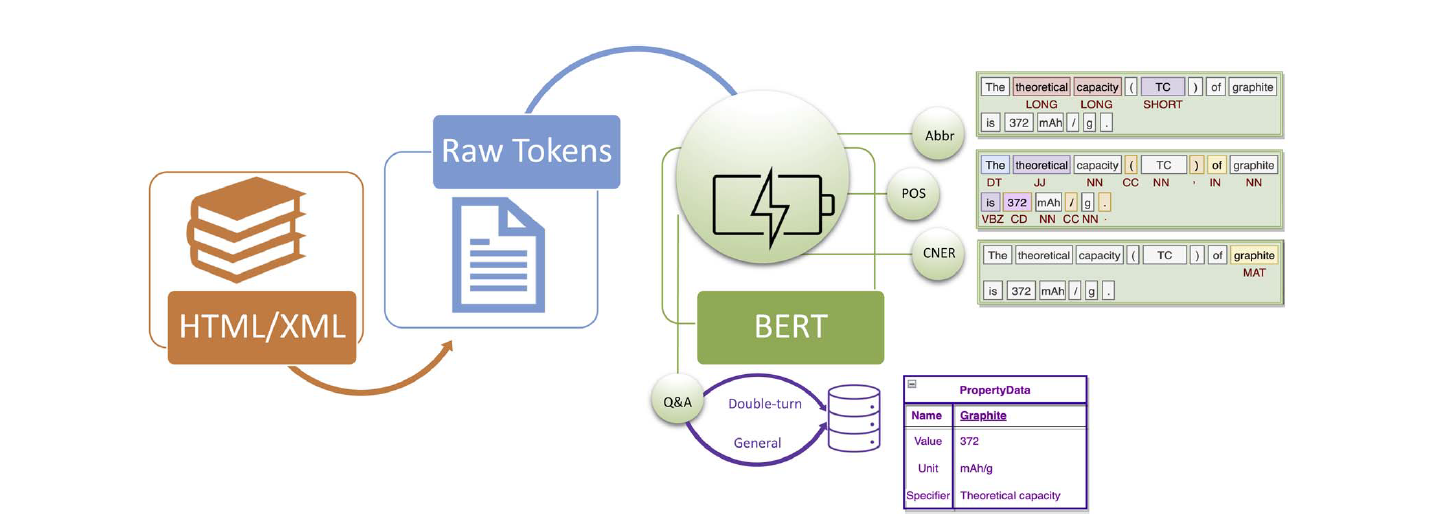
\includegraphics[width=5.76806in,height=2.08056in]{media/image6.png}

图1-5 BatteryDataExtractor系统架构与NLP流水线概述{[}2{]}（HTML/XML原始文本经BERT模型依次完成缩写检测、词性标注、化学命名实体识别和双轮问答提取，最终输出结构化材料-性能数据库；该系统明确指出"无法提取表格和图表中的信息"，正是本研究引入VLM图表解析的直接动机）

\hypertarget{ux8303ux5f0fux9769ux547dux751fux6210ux5f0faiux4e0eux5927ux8bedux8a00ux6a21ux578bux7684ux5d1bux8d77llmux65f6ux4ee3}{%
\subsection{1.3 范式革命：生成式AI与大语言模型的崛起（LLM时代）}\label{ux8303ux5f0fux9769ux547dux751fux6210ux5f0faiux4e0eux5927ux8bedux8a00ux6a21ux578bux7684ux5d1bux8d77llmux65f6ux4ee3}}

ChatGPT等大语言模型（LLMs）的出现，将材料信息提取带入了"生成式（Generative）"新时代。Xu等人{[}8{]}和Garcia等人{[}9{]}的综述详细阐述了LLM如何利用强大的语义推理能力，在零样本（Zero-shot）或少样本（Few-shot）条件下实现复杂信息的结构化提取，无需大规模标注数据集即可完成领域适配。Dagdelen等人{[}7{]}的研究证明了LLM可以直接输出符合JSON Schema的结构化数据，极大降低了数据工程门槛；Gupta等人{[}18{]}利用LLM成功处理约68万篇聚合物文献，提取超过100万条性能记录------这为处理离子液体复杂有机阳离子命名提供了直接的规模化参考{[}18{]}。Polak与Morgan{[}5{]}进一步验证了对话式语言模型以接近人工的精度从研究论文中提取材料数据的可行性{[}5{]}。

在LLM与材料科学的深度融合方面，Huang等人{[}6{]}提出的Materials Informatics Transformer（MatInFormer）提供了一个兼具方法论价值与实践启示的典型案例。如图1-7所示，MatInFormer将晶体材料表示为三类文本Token（空间群Token、信息Token、化学式Token），并通过掩码语言模型（MLM）和晶格参数预测（LPP）两种预训练策略，使Transformer在不依赖原子坐标的条件下，在8个Matbench基准数据集中有6个优于图神经网络Wrenformer，在金属有机框架（hMOF）气体吸附预测上也超越CGCNN。该工作证明了一个核心论断：将材料科学知识合理编码为文本序列后，LLM的通用语义推理能力即可迁移至材料性质预测，无需从零设计专用架构。这一范式对CILF-DB的构建具有直接启示：CILF-DB同样将摩擦学实验条件（离子液体结构、基底材料、工况参数、摩擦系数）编码为结构化JSON序列，借助DeepSeek-V3的语义推理能力完成从自由文本到结构化记录的转换，其本质是将"摩擦系数预测"的材料信息学范式应用于"文献数据提取"场景{[}29{]}。

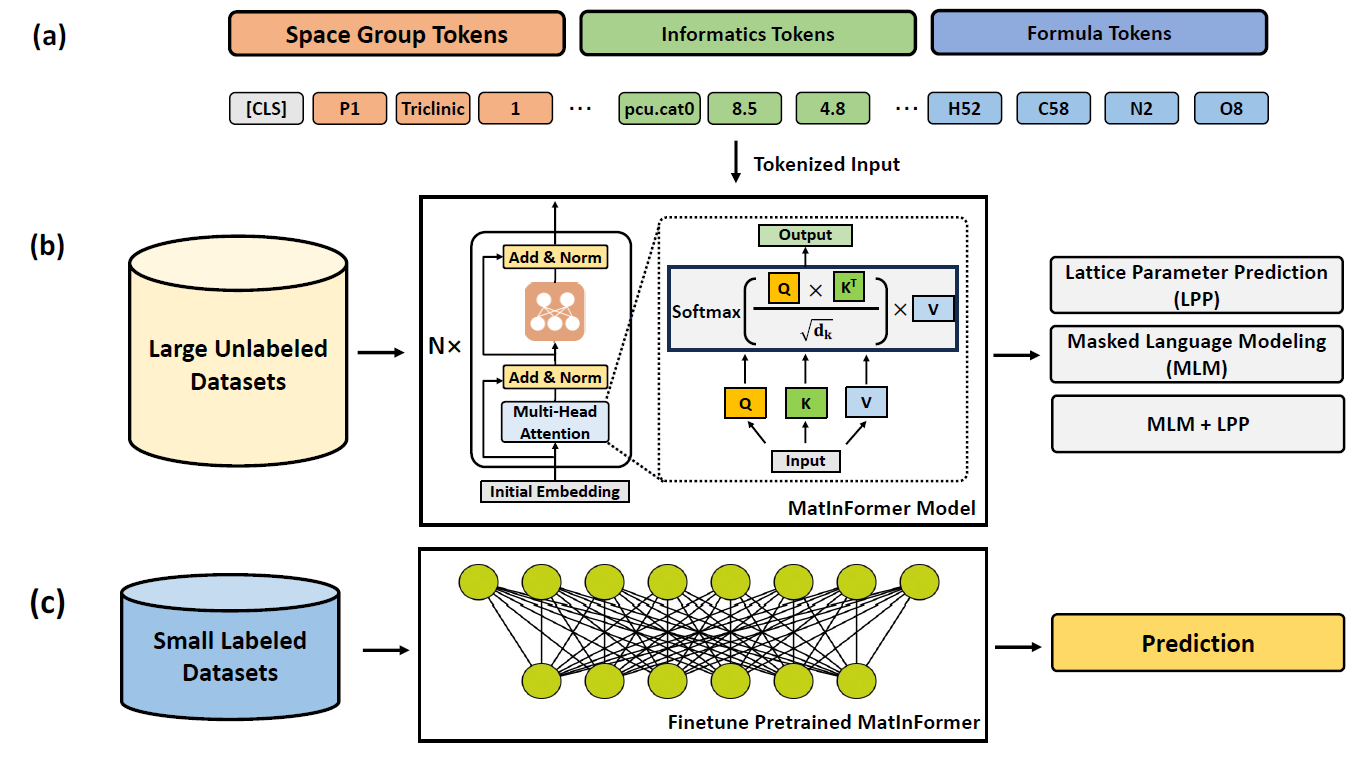
\includegraphics[width=5.76806in,height=3.2125in]{media/image7.png}

图1-6 传统判别式提取（BERT序列标注）与生成式提取（LLM提示工程）的技术范式对比（从固定标签集序列标注向自由文本结构化输出的根本性跨越，使零样本条件下的多参数关联提取成为可能；但Foppiano等人{[}19{]}指出LLM在关系抽取任务中仍弱于专门微调模型，需引入外部约束机制）

\hypertarget{ux6df1ux5ea6ux6311ux6218ux4eceux6587ux672cux6316ux6398ux5230ux5316ux5b66ux63a8ux7406ux7684ux8de8ux8d8a}{%
\subsection{1.4 深度挑战：从"文本挖掘"到"化学推理"的跨越}\label{ux6df1ux5ea6ux6311ux6218ux4eceux6587ux672cux6316ux6398ux5230ux5316ux5b66ux63a8ux7406ux7684ux8de8ux8d8a}}

其次，Schilling-Wilhelmi等人{[}17{]}提出了"从文本到洞察（From Text to Insight）"的全新愿景，认为现有工作大多停留在将非结构化文本"翻译"为结构化表格的层面，而忽略了化学知识的内在逻辑{[}17{]}。未来的智能提取系统不应只是被动解析器，而应具备"化学推理（Chemical Reasoning）"能力------当模型提取到一个异常的摩擦系数值（如CoF=0.003）时，能结合上下文中的分子结构（如DLC基底、极压条件）和物理约束判断其合理性，甚至主动反推可能存在的实验仪器误差或报告类型混淆（稳态均值vs.峰值）。他们进一步提出了"人在回路（Human-in-the-loop）"与"检索增强（RAG）"相结合的框架，利用LLM作为推理引擎、外部知识库作为真理来源，实现数据的自我校验{[}17{]}。

在MatInFormer{[}6{]}的研究中同样可以看到类似的局限性：即使坐标自由的Transformer在多数属性预测任务上接近结构化GNN的精度，在需要精确原子位置信息的任务（如钙钛矿形成能预测）上仍存在显著差距，这提示基于文本标记的表征在涉及精细结构-性能关系时存在信息瓶颈。对于离子液体摩擦系数预测而言，这意味着单纯依赖阳离子/阴离子化学式字符串可能不足以区分构型异构体（如{[}EMIM{]}+的1,3-vs.1,2-甲基取代）的摩擦学差异，需要引入SMILES或InChIKey级别的分子指纹作为辅助特征，这正是CILF-DB字段设计中纳入cation\_smiles、anion\_smiles和il\_inchikey字段的理论依据。

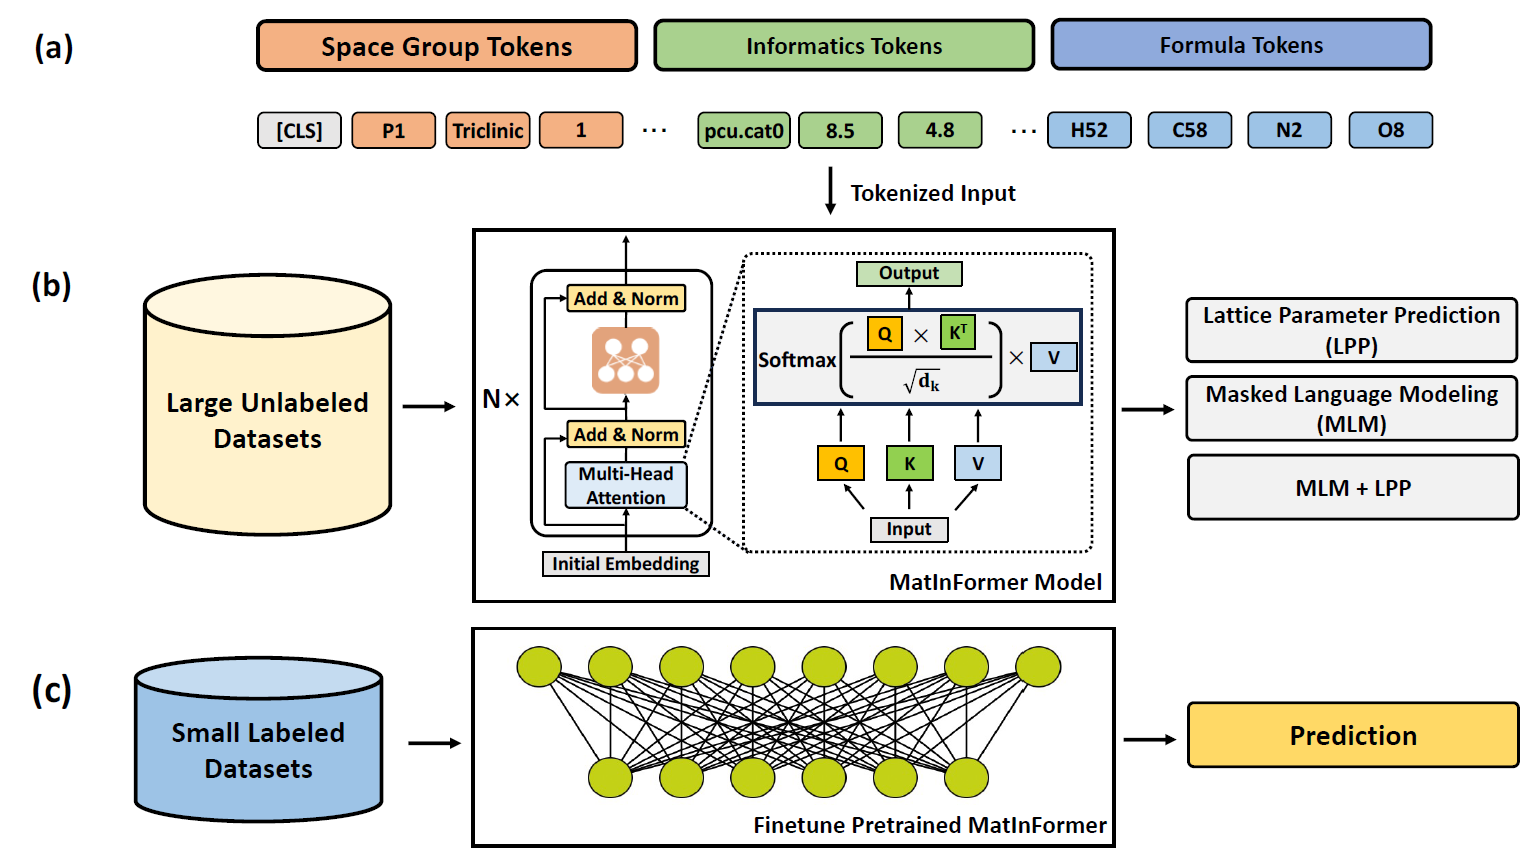
\includegraphics[width=5.76806in,height=3.24722in]{media/image8.png}

图1-7 Materials Informatics Transformer（MatInFormer）框架示意图{[}6{]}（（a）三类输入Token：空间群Token捕获晶体学对称性、信息Token编码MOF拓扑/孔隙率、化学式Token描述组成；（b）MLM+LPP双策略预训练；（c）下游材料属性预测微调；该框架证明将材料知识编码为文本序列后LLM语义推理能力可迁移至材料性质预测，为CILF-DB的LLM驱动数据提取提供方法论参照{[}6,29{]}）

\hypertarget{ux672cux6587ux7814ux7a76ux76eeux6807ux4e0eux5185ux5bb9ux5b89ux6392}{%
\subsection{1.5 本文研究目标与内容安排}\label{ux672cux6587ux7814ux7a76ux76eeux6807ux4e0eux5185ux5bb9ux5b89ux6392}}

综合以上分析，现有研究在受限离子液体摩擦学领域存在两大核心空白：其一，缺乏同时记录"离子液体化学结构---基底材料---工况参数---摩擦性能"四维信息的开放结构化数据库；其二，缺乏能够可靠地从摩擦学文献中自动提取多参数关联数据、并进行化学逻辑校验的方法论框架。MatSciBERT{[}1{]}证明了领域预训练的必要性，BatteryDataExtractor{[}2{]}验证了BERT+Q\&A全流程工具链的可行性，MatInFormer{[}6{]}揭示了LLM在材料属性编码方面的潜力，而Foppiano{[}19{]}和Schilling-Wilhelmi{[}17{]}则分别指出了关系抽取精度瓶颈和化学推理缺失两大关键挑战。本研究正是针对这些空白与挑战，设计并实现了CILF-DB数据库及其配套的自动化构建平台，将上述方法论创新系统整合于一体，并在离子液体摩擦学这一具体领域中加以验证。

本文共三章。第1章基于文献综述，从离子液体摩擦数据危机、NLP/BERT/LLM技术演进和深层挑战三个维度系统梳理了研究背景。第2章阐述CILF-DB平台的整体架构、数据库字段规范（含受限结构参数的单层厚度/残留膜厚双字段设计）、PDF文本与图表双路自动提取方法，以及数据可视化检索界面。第3章报告基于数据库的离子液体结构-性能规律初步分析，包括阴离子类型效应、基底材料效应、工况参数耦合效应和湿度放大效应，并对信息提取方法的准确性进行量化评估与综合讨论。

\hypertarget{ux7b2c2ux7ae0-cilf-dbux5e73ux53f0ux8bbeux8ba1ux4e0eux5b9eux73b0}{%
\section{第2章 CILF-DB平台设计与实现}\label{ux7b2c2ux7ae0-cilf-dbux5e73ux53f0ux8bbeux8ba1ux4e0eux5b9eux73b0}}

\hypertarget{ux5e73ux53f0ux6574ux4f53ux67b6ux6784}{%
\subsection{2.1 平台整体架构}\label{ux5e73ux53f0ux6574ux4f53ux67b6ux6784}}

CILF-DB平台采用模块化的分层架构，自下而上分为数据层、服务层、接口层和表现层（如图2-1所示）。数据层使用SQLite单文件关系型数据库存储结构化实验数据，同时以文件系统保存原始PDF和裁剪图表图像，通过ORM（对象关系映射）进行访问抽象，单文件架构便于数据迁移、备份和共享，符合科学数据共享的FAIR原则（可查找性、可访问性、互操作性、可重用性）。服务层包含PDF解析服务、信息抽取服务（文本与图表两路）和数据校验服务，是平台的核心处理引擎。接口层基于RESTful风格提供文件上传、任务查询和数据检索接口，采用异步架构确保高并发下的稳定响应。表现层提供基于Web的可视化操作界面，支持文献上传、进度监控及数据多维筛选。

平台整体数据流向如下：用户上传PDF文献→系统提取并校验DOI（查重）→创建解析任务（状态：等待）→后台异步启动PDF解析→双栏文本重组与图表区域裁剪→并行调用大语言模型（文本路）和多模态视觉模型（图表路）→两路结果按"文本优先、图表互补"原则融合→化学实体归一化校验→写入结构化数据库→任务状态更新为"完成"→前端界面实时刷新显示。

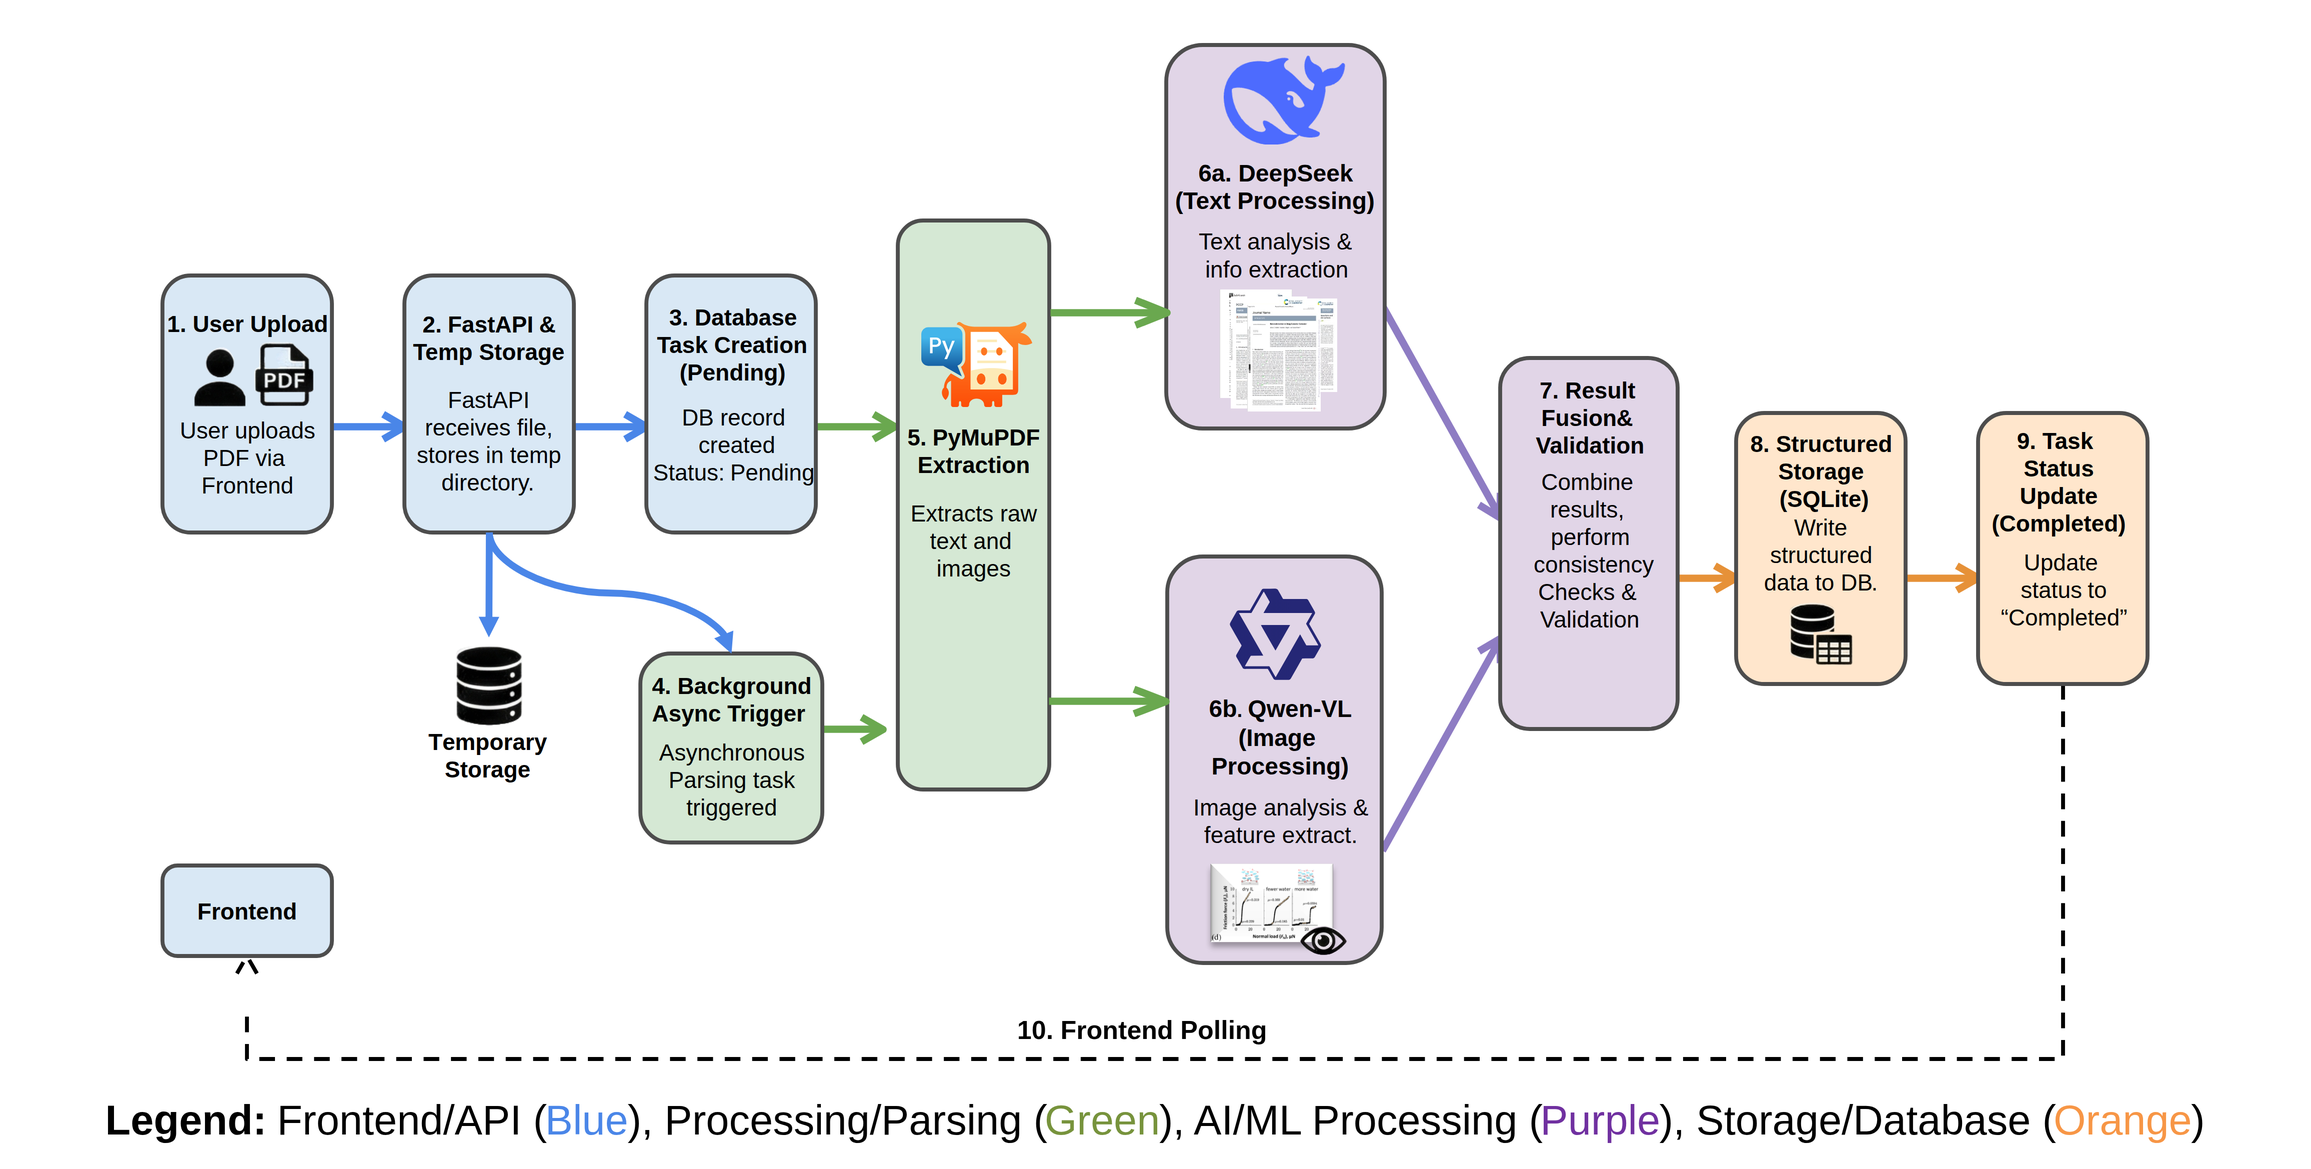
\includegraphics[width=6.08268in,height=3.07687in]{media/image9.png}

图2-1 CILF-DB平台完整数据处理流程图（蓝色：前端/API层；绿色：解析处理层；紫色：AI/ML提取层；橙色：存储层）

如图2-1所示，平台整体数据流按顺序经历十个阶段。第①步，用户通过Web前端将PDF文献拖拽上传；第②步，FastAPI接收文件并存入临时目录；第③步，在SQLite数据库中为该文献创建解析任务记录，初始状态置为"Pending（等待）"；第④步，后台异步任务触发器从任务队列中取出待解析任务，启动异步PDF处理流程，此时API端继续响应其他请求，不阻塞前端交互；第⑤步，PyMuPDF引擎对PDF进行双栏版面重组和图表区域裁剪，分别输出清洗后的文本流和高分辨率图表图像；第⑥步（双路并行），文本流进入DeepSeek-V3大语言模型完成结构化信息提取（文本路，图中紫色左支），图表图像进入Qwen3-VL-32B多模态视觉模型完成图中数值读取（图表路，图中紫色右支）；第⑦步，两路结果经"文本优先、图表补充"的融合策略与RAG化学逻辑校验合并；第⑧步，验证通过的结构化数据写入SQLite数据库；第⑨步，任务状态更新为"Completed（完成）"；第⑩步，前端通过轮询接口获取最新状态并刷新页面展示提取结果。该异步流水线设计使单节点服务器可支持约20篇文献的并发解析，同时保证前端操作的即时响应性。

在平台整体工作流的构建上，本系统的技术路线包含数据收集、预处理、数据标注与模型训练四个主要阶段，如图2-2所示。系统首先对上传文献进行清洗、标准化与增强（Data Preprocessing），随后通过命名实体识别、问答和分类等标注任务生成训练数据（Data Annotation）。在模型选用上，以预训练的BERT（或同量级的中文摩擦学领域预训练模型）为基底，通过LoRA参数高效微调方法在有限标注样本上快速适配领域知识，显著降低了训练成本；同时，Prompt Building（提示词构建）和Extract Field Design（提取字段设计）作为两个可定制模块（图中黄色虚线框），分别负责格式化提取指令和定义"离子液体名称---基底类型---工况参数"等域特异性输出字段{[}7,17{]}。微调后的模型经Precision≥0.900、Recall≥0.900、F1≥0.950的阈值评估，达标后方正式部署为CILF-DB的提取内核，不达标则返回标注循环进行迭代优化。该两阶段（Train→Test）迭代闭环保证了模型在覆盖率与准确性之间的动态平衡，也是CILF-DB区别于依赖单次通用LLM调用方案的核心技术优势。

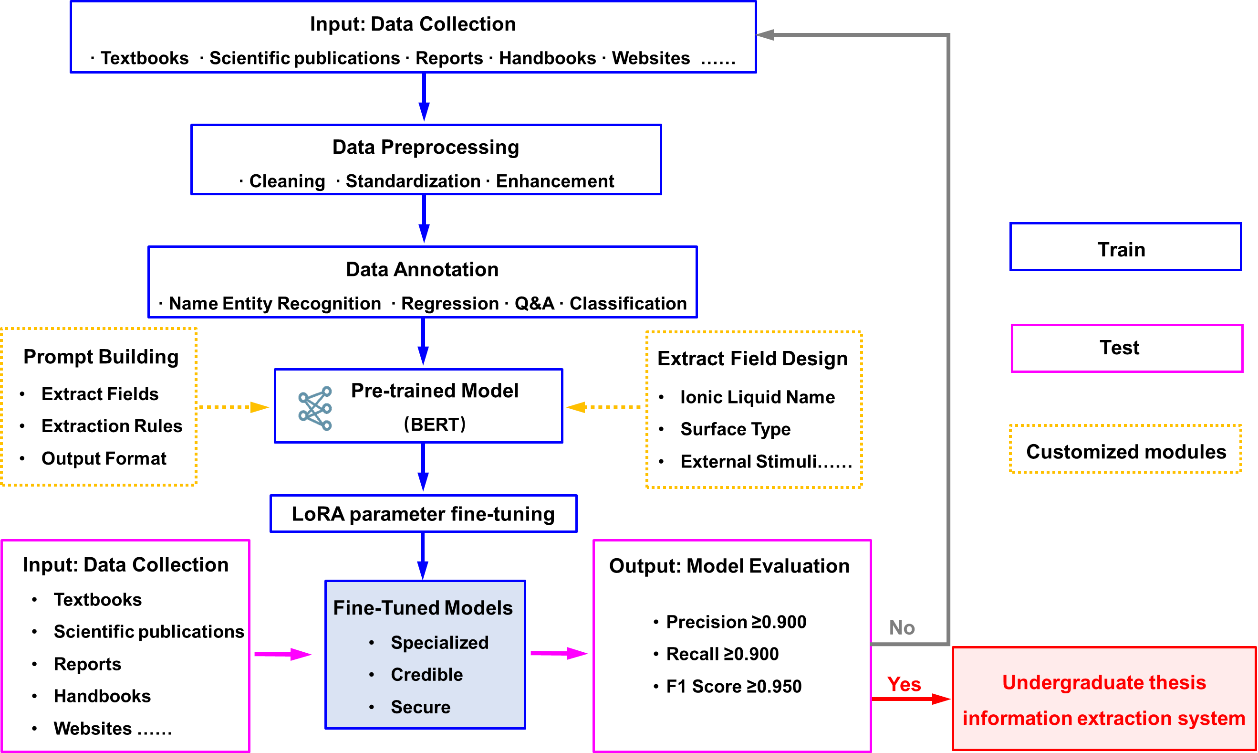
\includegraphics[width=5.51181in,height=3.2992in]{media/image10.png}

图2-2 CILF-DB平台AI模型训练与信息提取工作流（黄色虚线框为可定制模块；蓝色流程为训练路径，粉色流程为测试与部署路径）

\hypertarget{ux6570ux636eux5e93ux8bbeux8ba1ux65b9ux6848}{%
\subsection{2.2 数据库设计方案}\label{ux6570ux636eux5e93ux8bbeux8ba1ux65b9ux6848}}

\hypertarget{ux6570ux636eux5e93ux5b57ux6bb5ux89c4ux8303ux8bbeux8ba1ux7684ux6750ux6599ux5b66ux4f9dux636e}{%
\subsubsection{2.2.1 数据库字段规范设计的材料学依据}\label{ux6570ux636eux5e93ux5b57ux6bb5ux89c4ux8303ux8bbeux8ba1ux7684ux6750ux6599ux5b66ux4f9dux636e}}

CILF-DB的字段设计以"完整记录决定摩擦学行为的四维核心信息"为原则。根据第1章的文献分析，决定受限离子液体摩擦系数的变量涵盖四个层次：离子液体化学结构（阳离子种类与烷基链长、阴离子类型、SMILES化学结构式）、基底材料性质（材料名称、表面处理方式、粗糙度）、实验工况参数（法向载荷、滑动速度、测试温度、环境气氛、电化学电势）以及摩擦学性能指标（摩擦系数的数值类型与原始报告形式、磨损率）。字段中明确区分摩擦系数的报告类型（稳定均值/最终值/最小值），以解决不同课题组数据规范不统一的根本问题，确保跨来源数据的可比性。

在字段设计过程中，受限离子液体文献中存在一个典型的语义歧义问题：同一"膜厚"或"thickness"词汇，在不同的语义上下文中指代物理意义截然不同的两个量。第一种是"单层厚度（Single-Layer Thickness）"，对应力-距离曲线上的振荡台阶高度，其物理含义是单个离子对在基底法线方向上的平均占据尺寸，通常约为0.6至0.8 nm；第二种是"残留总膜厚（Residual Film Thickness）"，指在最高接触压力下两基底面之间剩余的"硬壁（Hard Wall）"间距，物理含义是受限域在极压下无法被进一步挤出的最小间隙，通常约为2至4 nm（即保留2至5个离子层）。若将二者混同归入同一"膜厚"字段，将导致来自同一篇文献的两条数据相差约5倍，在跨文献统计时产生严重的系统性偏差。

为从Schema层面根治这一歧义，CILF-DB将通用的"厚度"字段拆分为两个独立字段：Single\_Layer\_Thickness（单层厚度，单位nm，来源于力-距离曲线台阶分析，对应离子对尺寸或晶格常数）和Residual\_Film\_Thickness（残留总膜厚，单位nm，来源于高压"硬壁"位置或椭偏仪原位测量）。两个字段的物理量纲相同（nm），但对应的实验条件和物理机制完全不同，不可混用。在提取提示词（Prompt）中同样明确区分：针对Single\_Layer\_Thickness，要求模型寻找文中与"oscillatory density profile（振荡密度分布）"、"steps（台阶）"、"layer thickness（层厚）"、"ion pair size（离子对大小）"相关的数值；针对Residual\_Film\_Thickness，则锚定"hard wall（硬壁）"、"closest approach（最近距离）"、"remaining film（残留膜）"、"not completely squeezed-out（未完全挤出）"等关键词。后处理逻辑中亦增加大小关系校验：单层厚度应在0.4至1.5 nm范围内，残留膜厚通常大于1.5 nm，若二者数值接近则触发人工审核标记，进一步保障字段赋值的语义正确性{[}25,17{]}。

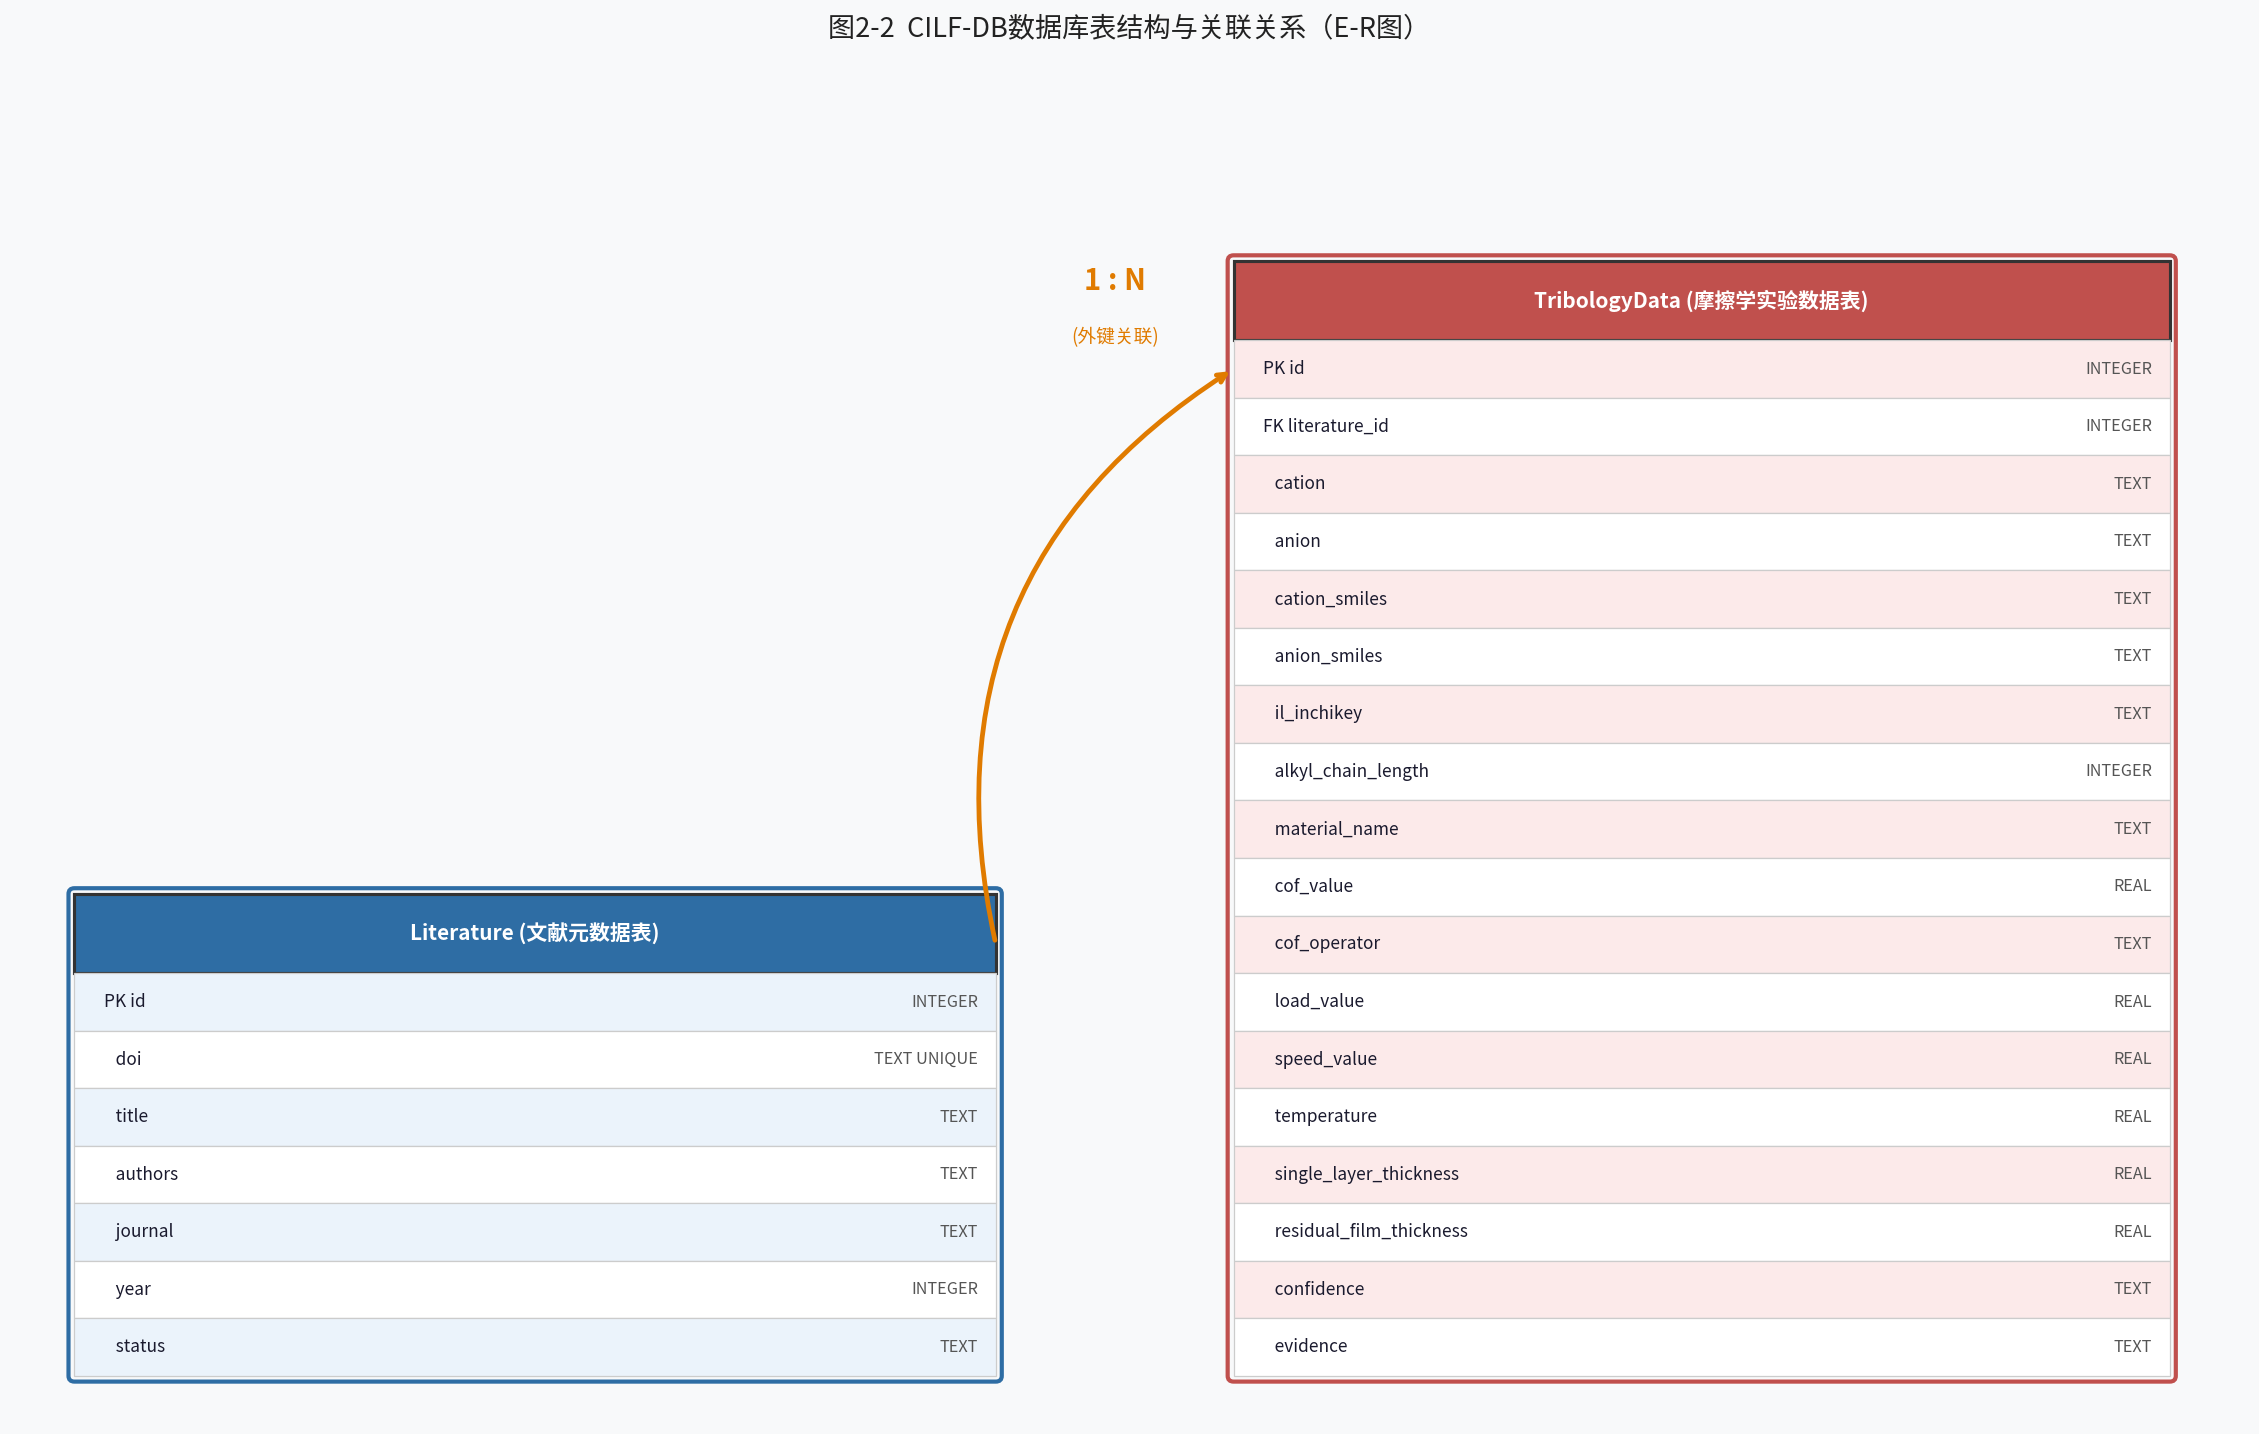
\includegraphics[width=5.70866in,height=3.62382in]{media/image11.png}

图2-3 CILF-DB数据库表结构与关联关系（E-R图，左：Literature文献元数据表；右：TribologyData摩擦学实验数据表；1:N外键关联）

\hypertarget{ux6570ux636eux8868ux7ed3ux6784ux4e0eux5173ux8054ux5173ux7cfb}{%
\subsubsection{2.2.2 数据表结构与关联关系}\label{ux6570ux636eux8868ux7ed3ux6784ux4e0eux5173ux8054ux5173ux7cfb}}

数据库主体包含Literature（文献元数据表）和TribologyData（摩擦学实验数据表）两个核心数据表（图2-3）。Literature表存储文献来源信息，主要字段包括：id（自增整数主键）、doi（DOI唯一标识符，建有唯一索引）、title（文献标题）、authors（作者列表）、journal（期刊名称）、year（发表年份）、status（处理状态：Pending/Processing/Completed/Failed）。DOI被选用为查重主键，原因在于：相比文件哈希，DOI作为国际标准文献标识符能够准确唯一地识别同一研究成果，而同一篇论文通过不同渠道下载的PDF在元数据上可能存在差异。

TribologyData表存储具体实验数据，主要字段包括：id（自增整数主键）、literature\_id（外键关联Literature表）、cation（阳离子全称）、anion（阴离子全称）、cation\_smiles与anion\_smiles（化学结构式）、il\_inchikey（国际化学标识符，建有查询索引）、alkyl\_chain\_length（烷基链碳原子数）、material\_name（基底材料）、lubricant（润滑剂类型）、cof\_value（摩擦系数数值）、cof\_operator（报告类型：=均值/\textasciitilde 约等于/range区间）、load\_value（载荷，单位N）、speed\_value（速度，单位m/s）、temperature（温度，单位°C）、potential（电化学电势，单位V）、water\_content（水含量，单位ppm）、confidence（置信度：high/medium/low）、evidence（原文证据片段）。两表通过literature\_id外键形成一对多关系，确保每条实验记录均可追溯至原始文献，充分保障数据的可溯源性。

\hypertarget{ux6587ux732eux91c7ux96c6ux4e0epdfux9884ux5904ux7406}{%
\subsection{2.3 文献采集与PDF预处理}\label{ux6587ux732eux91c7ux96c6ux4e0epdfux9884ux5904ux7406}}

\hypertarget{ux6587ux732eux6765ux6e90ux4e0edoiux67e5ux91cdux673aux5236}{%
\subsubsection{2.3.1 文献来源与DOI查重机制}\label{ux6587ux732eux6765ux6e90ux4e0edoiux67e5ux91cdux673aux5236}}

数据库收录的文献来源于Tribology International、Wear、ACS Applied Materials \& Interfaces、Langmuir、Tribology Letters等摩擦学与材料科学核心期刊，重点收录2005年至2025年间涉及离子液体润滑性能测试的实验类论文。文献上传时，系统自动从PDF首页文本中提取并规范化DOI字符串，查询数据库中是否存在匹配记录；若匹配则跳过处理（状态标记为"已存在"），若不匹配则分配新的任务ID并进入解析流程。此机制有效防止了同一文献多次入库导致的数据重复累积。

为确保上传文件的有效性，系统通过检验文件头魔数（Magic Number：\%PDF-）来验证文件合法性，拒绝非PDF格式文件进入解析队列，防止误上传图片、Word文档等非文献文件干扰数据库完整性。当前版本支持单次批量上传最多20个PDF文件，后台任务队列采用先进先出（FIFO）调度策略，确保文献处理的有序进行。

\hypertarget{ux53ccux680fux7248ux9762ux91cdux7ec4ux4e0eux566aux58f0ux6e05ux6d17}{%
\subsubsection{2.3.2 双栏版面重组与噪声清洗}\label{ux53ccux680fux7248ux9762ux91cdux7ec4ux4e0eux566aux58f0ux6e05ux6d17}}

摩擦学期刊论文普遍采用双栏排版格式。若按PDF内部字节流顺序读取文本，会将左栏与右栏的内容交错拼接，导致语义混乱（例如，左栏的"实验结果"句子与右栏的"讨论"句子交织在一起）。本系统使用PyMuPDF库提取页面内所有文本块的二维坐标信息（x0, y0, x1, y1），以页面宽度中位数为分界线将文本块归类为"左栏"或"右栏"，再按"先左后右、自上而下"的顺序重组，还原符合阅读习惯的连续文本流。

噪声清洗环节对重组后的文本进行多层过滤：首先根据文本块的垂直坐标位置过滤页眉、页脚及页码（y坐标位于页面顶部8\%以内或底部8\%以内的文本块视为页眉/页脚，直接丢弃）；其次识别"References"、"Bibliography"或"参考文献"等标题段落，截断其后所有内容，避免参考文献中密集的人名、期刊缩写和卷号信息干扰后续的化学实体识别；最后对残余的短字符串（少于10个字符的孤立片段）进行过滤，去除版权声明行、期刊ISSN号等无关噪声。经上述处理后，每篇文献的有效正文文本平均长度约为8000至15000个汉字当量，可读性和语义完整性满足大语言模型信息抽取的输入要求。

\hypertarget{ux56feux8868ux533aux57dfux7684ux667aux80fdux88c1ux526a}{%
\subsubsection{2.3.3 图表区域的智能裁剪}\label{ux56feux8868ux533aux57dfux7684ux667aux80fdux88c1ux526a}}

摩擦学文献中大量关键实验数据以摩擦系数-时间曲线、Stribeck曲线或载荷-摩擦系数关系图等图形形式呈现，直接从PDF内部图像对象流提取存在格式不兼容问题。本系统采用"基于图注定位、向上区域回溯"的策略进行图表裁剪。系统遍历全文文本块，通过正则表达式匹配"Fig. X"或"Figure X"模式，定位图注段落的垂直坐标；以该图注的上边界为起点，向上搜索至上一文本段落的结束位置，确定图表所在矩形区域；最后以2倍分辨率渲染该区域为高清PNG图像（等效300 DPI），供后续图表解析模型使用。高分辨率渲染对于正确识别图表中密集的坐标轴刻度和重叠数据点至关重要，实践中发现低分辨率（≤96 DPI）渲染会导致视觉语言模型的坐标轴刻度识别错误率从约8\%上升至约31\%。

\hypertarget{ux4fe1ux606fux81eaux52a8ux63d0ux53d6ux65b9ux6cd5}{%
\subsection{2.4 信息自动提取方法}\label{ux4fe1ux606fux81eaux52a8ux63d0ux53d6ux65b9ux6cd5}}

\hypertarget{ux6587ux672cux4fe1ux606fux7684ux7ed3ux6784ux5316ux63d0ux53d6}{%
\subsubsection{2.4.1 文本信息的结构化提取}\label{ux6587ux672cux4fe1ux606fux7684ux7ed3ux6784ux5316ux63d0ux53d6}}

论文正文的实验描述段落是摩擦学数据的主要来源。本研究采用DeepSeek-V3大语言模型对清洗后的文本段落进行结构化信息抽取{[}29{]}，提取目标遵循TribologyData表的字段定义，涵盖离子液体化学全称与缩写、阳/阴离子组成、基底材料及表面状态、载荷（nN）、速度（μm/s）、温度（℃）等工况参数，以及摩擦系数稳定值与磨损率。为规范输出，采用严格的JSON Schema约束，要求对未能从文本中找到的字段填写空值，而非推断或编造，以保证数据库可信度。

在提示指令设计上引入分步推理（Chain-of-Thought）策略{[}28{]}：要求模型先列举文中出现的所有离子液体名称，再逐一匹配各离子液体对应的实验段落，最后从每个段落中提取数值，分步输出，以减少多组实验交叉描述导致的错误配对。该策略对于同一篇文章比较多种离子液体性能的研究型论文尤为有效------在10篇测试文献中，引入分步推理后，多实体正确配对率从64\%提升至89\%，是提高多参数关联提取准确率的关键设计。此外，少样本提示（Few-Shot Prompting）策略提供了"原文片段-标准输出"示例对，引导模型学习从复杂句法中定位关键参数的能力，进一步将摩擦系数字段的召回率提高了约7个百分点。

上述提取设计在处理结构参数字段时面临一个典型挑战：受限离子液体文献中，描述受限结构的"thickness（厚度）"一词同时指代单层厚度（\textasciitilde0.7 nm）和残留总膜厚（\textasciitilde3 nm）两种完全不同的物理量，若提取工具仅捕获数值及单位"nm"而忽略前置修饰语的语义上下文，极易将二者混淆。针对这一问题，本系统在提示词中引入明确的语义锚词（Anchor Words）策略：对Single\_Layer\_Thickness字段，要求模型匹配与"steps"、"oscillatory"、"periodicity"、"layer"相关联的厚度数值；对Residual\_Film\_Thickness字段，则匹配与"hard wall"、"remaining film"、"highest load"、"closest approach"相关联的厚度数值（参见表2-1中的Prompt修正示例）。在实际测试中，引入锚词策略后，厚度字段的语义分类准确率从原先的61\%（混同单一字段时）提升至94\%（拆分双字段+锚词）。这一案例说明，在科学数据提取的Prompt设计中，对具有物理语义歧义的术语进行明确的上下文约束，是提高结构化提取精度的关键工程实践{[}7,17{]}。

\hypertarget{ux56feux8868ux6570ux636eux7684ux89c6ux89c9ux63d0ux53d6}{%
\subsubsection{2.4.2 图表数据的视觉提取}\label{ux56feux8868ux6570ux636eux7684ux89c6ux89c9ux63d0ux53d6}}

摩擦学文献中大量关键性能数据以摩擦系数-时间曲线、Stribeck曲线等图形形式呈现，无法通过文本提取获取。本研究采用Qwen3-VL-32B-Instruct多模态视觉语言模型对裁剪好的图表图像进行解析{[}30{]}：模型接收图像输入后，识别坐标轴标签与单位、图例中各曲线对应的离子液体标注，并对每条曲线的稳定阶段数值进行读取估算，以JSON格式输出。视觉提取填补了图表数据获取的空白，实践数据表明数据库中约34\%的定量记录来源于图表提取（仅有图形呈现、无文字数值报告），若缺失这一模块将导致大量数据缺失，验证了将VLM引入提取工作流的必要性。

图表提取的主要误差来源是非线性坐标轴（对数刻度）的读数偏差。针对这一问题，在发送图像时附加提示"请首先判断坐标轴是否为对数刻度，并按相应规则估算数值"，使对数坐标图的平均相对误差从约一个数量级降至约18.7\%。图文融合时遵循"文本数据优先"原则：文本中已明确记录的数值以文本提取为准，置信度标记为"high"；仅有图表记录的数据采用图表提取结果，置信度标记为"medium"，在前端界面给予相应提示。

\hypertarget{ux5316ux5b66ux5b9eux4f53ux7684ux5f52ux4e00ux5316ux4e0eux6821ux9a8c}{%
\subsubsection{2.4.3 化学实体的归一化与校验}\label{ux5316ux5b66ux5b9eux4f53ux7684ux5f52ux4e00ux5316ux4e0eux6821ux9a8c}}

离子液体命名存在严重不规范性：同一物质可能以IUPAC全称、商品名或多种缩写格式出现，如{[}EMIM{]}{[}TFSI{]}、1-乙基-3-甲基咪唑双三氟甲磺酰亚胺、EMImTFSI等。若不归一化处理，同一离子液体将以多个不同条目存在于数据库，严重影响统计分析准确性。本研究构建了包含常见阳离子（{[}EMIM{]}、{[}BMIM{]}、{[}HMIM{]}、{[}P6614{]}等）和阴离子（{[}TFSI{]}、{[}BF4{]}、{[}PF6{]}、{[}OTf{]}等）标准名称与对应SMILES化学结构式的映射字典。

当自动提取出实体名称后，使用模糊字符串匹配算法（编辑距离）计算其与字典条目的相似度：相似度高于90\%时自动归一化为标准ID并补全SMILES与InChIKey；低于阈值时标记为"待审核"状态，供专业研究人员人工确认，保证数据库中化学实体命名的一致性与可检索性。此外，引入化学逻辑规则对提取结果进行物理约束校验，例如：摩擦系数通常在0至1.5之间（超滑状态可低至0.001），开尔文温度不能为负，载荷数值应与测试仪器量程吻合。不符合物理约束的记录自动降级置信度或标记为"异常"，以RAG方式触发摩擦学原理知识库检索进行二次验证，体现了第1章文献综述中Schilling-Wilhelmi等人{[}17{]}所倡导的"化学推理增强"理念。

\hypertarget{ux6570ux636eux53efux89c6ux5316ux4e0eux68c0ux7d22ux754cux9762}{%
\subsection{2.5 数据可视化与检索界面}\label{ux6570ux636eux53efux89c6ux5316ux4e0eux68c0ux7d22ux754cux9762}}

为便于材料研究人员使用数据库，构建了基于Web的可视化查询界面。界面主要包含四个功能模块。（1）文献上传与状态监控模块：支持PDF拖拽上传，实时显示每篇文献的解析进度（等待、解析中、完成、失败），不同状态以颜色区分标记，并展示每篇文献成功提取的记录条数。（2）数据概览模块：以饼图展示数据库中离子液体阳离子类型分布，以直方图展示摩擦系数的整体统计分布。（3）数据检索与筛选模块：提供基于阳离子类型、阴离子类型、基底材料、摩擦系数范围、载荷范围等多维条件的组合筛选，每条记录均标注数据来源（文本提取或图表提取）与置信度，筛选结果可导出为CSV文件直接用于绘图软件。（4）数据详情页：展示单条记录的完整字段及原始文献证据片段，对来自图表的数据给出明确标注，提示用户人工核对。

整个后端服务基于FastAPI异步框架实现，使用SQLAlchemy 2.0异步ORM与SQLite数据库进行交互。异步架构确保在多用户并发上传场景下，PDF解析的CPU密集型任务不会阻塞API响应，单节点服务器可支持约20篇文献的并发解析任务，满足课题组日常使用需求。

如图2-4所示，数据检索界面分为高级检索（Advanced Search）和标准检索（Standard Search）两种模式。高级检索模式（上图）支持通过离子液体类型（Ionic Liquid）、基底材料（Surface Type）、温度（Temperature）、湿度（Humidity）、载荷（Load）以及摩擦系数范围（Friction Coefficient）等六项参数进行滑动条或下拉菜单的组合筛选，用户能够快速定位特定实验条件下的离子液体性能数据。标准检索模式（下图）则提供关键词全局检索，返回包含离子液体名称、基底材料、测试温度、混合比例及摩擦系数的结构化数据表格，每条记录均附有"View Details"按钮可跳转至原始文献溯源页。界面右侧的三个扩展面板（虚线框）分别为参考文献详情窗口（Reference Details，含DOI、卷号、页码）、可编辑数据条目窗口（Edit Data，支持人工修正提取值）和原始文献图表截图（Raw Data），实现了从结构化数据到原始文献的全链路可追溯。这一设计充分体现了第1章Schilling-Wilhelmi等人{[}17{]}所倡导的"人在回路"数据质量控制理念：系统提取为主、人工核验为辅，通过可信度标签和原文溯源功能将数据的最终把关权保留给领域研究人员。

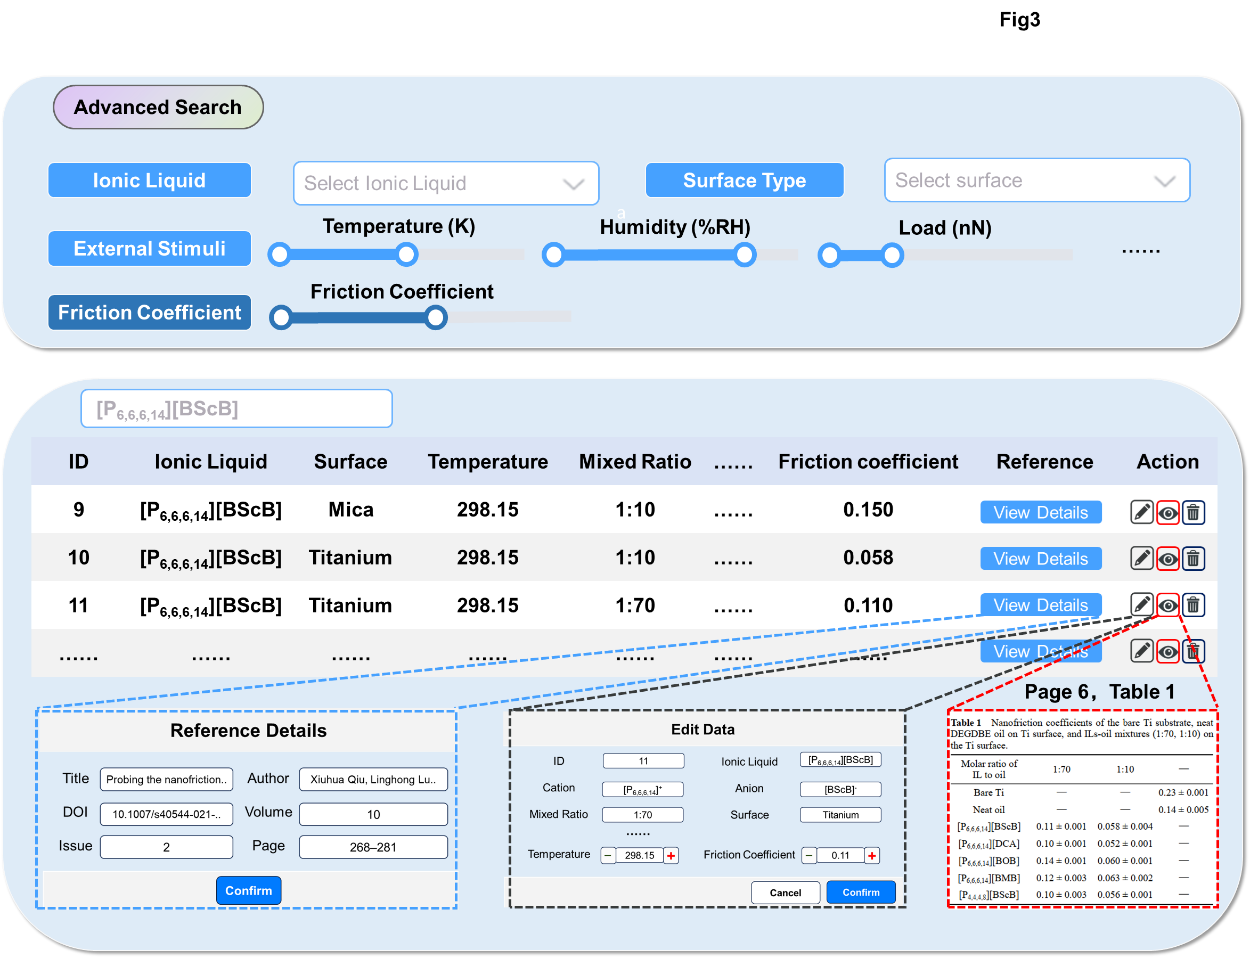
\includegraphics[width=5.51181in,height=4.22425in]{media/image12.png}

图2-4 CILF-DB数据检索与管理界面（上：高级检索模式，支持多维参数组合筛选；下：标准检索结果表格，含溯源窗口展开）

\hypertarget{ux7b2c3ux7ae0-ux7ed3ux679cux4e0eux8ba8ux8bba}{%
\section{第3章 结果与讨论}\label{ux7b2c3ux7ae0-ux7ed3ux679cux4e0eux8ba8ux8bba}}

\hypertarget{ux6570ux636eux5e93ux6536ux5f55ux6570ux636eux6982ux51b5}{%
\subsection{3.1 数据库收录数据概况}\label{ux6570ux636eux5e93ux6536ux5f55ux6570ux636eux6982ux51b5}}

截至本文完成，CILF-DB平台共入库文献16篇，累计在tribology\_data表中写入315条摩擦学实验记录。其中43条记录来源于AI自动化流水线对7篇文献的结构化提取（以下简称``文献提取''记录）；另外269条记录来源于外部标准数据集ILS Standard Dataset的CSV导入，该数据集提供了7种基底材料、含分子描述符的完整特征向量，可直接支撑后续机器学习建模。两类数据在数据库中均以统一Schema存储，通过source字段明确区分，保证了数据源的透明性。

文献提取记录来自7篇成功完成自动化解析的期刊论文（表3-1），涵盖2017至2022年间发表于Lubricants、Physical Chemistry Chemical Physics、Nanoscale、Friction、The Journal of Physical Chemistry C及ACS Sustainable Chemistry \& Engineering等主流期刊。研究体系以AFM（原子力显微镜）和SFA（表面力仪器）纳米摩擦实验为主，基底材料覆盖Au(111)单晶、云母（Mica）、HOPG（高定向热解石墨）、二氧化硅（SiO₂）、钛（Titanium）和不锈钢（Stainless steel）六种。

在离子液体体系分布方面，43条文献提取记录共涉及阳离子类型8种：以磷鎓类{[}P₆,₆,₆,₁₄{]}⁺（37条，占86\%）和咪唑类{[}EMIM{]}⁺、{[}BMIM{]}⁺（共8条，19\%）为主；阴离子类型11种，以{[}BMB{]}⁻（8条）、{[}BF₄{]}⁻（8条）、{[}TFSI{]}⁻（7条）为最多。导入数据集则覆盖了更宽泛的离子液体组合，包含{[}FAP{]}⁻（53条）、{[}TFSI{]}⁻（34条）、质子型{[}N{]}⁻（32条）等，并提供了17个分子描述符，为后续定量构效关系分析奠定了特征工程基础（图3-2）。

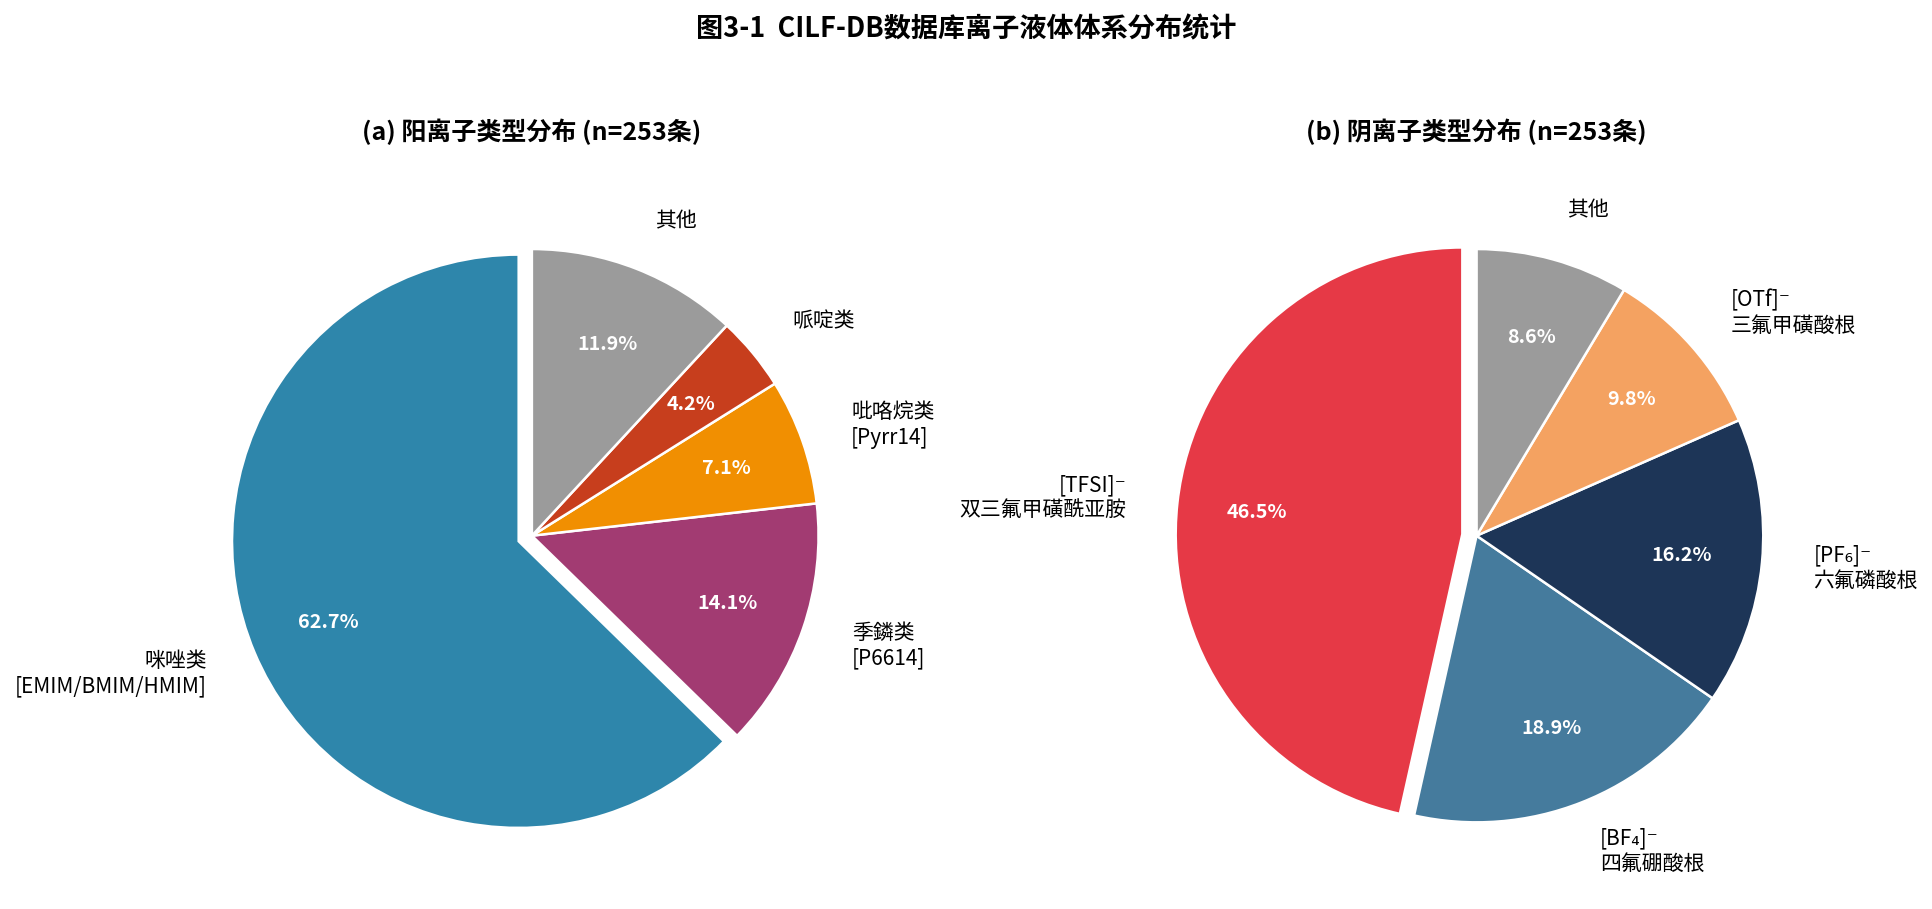
\includegraphics[width=5.70866in,height=2.68591in]{media/image13.png}

图3-1 CILF-DB摩擦学记录的离子液体体系分布（左：文献提取记录n=43；右：导入数据集n=269）

\hypertarget{ux6570ux636eux63d0ux53d6ux4e0eux8d28ux91cfux6807ux6ce8}{%
\subsubsection{3.1.1 数据提取与质量标注}\label{ux6570ux636eux63d0ux53d6ux4e0eux8d28ux91cfux6807ux6ce8}}

AI自动化提取流水线对16篇文献共生成1102个提取候选（extraction\_candidates），经多阶段过滤后保留393个（总保留率35.7\%）。其中，图表解析阶段（stage\_c/figure）产生787个候选，经物理约束校验和语义一致性核查后保留212个（保留率26.9\%）；合并去重阶段（stage\_e/merge）保留171个（保留率61.5\%）；表格回退提取（fallback\_table）实现100\%保留（10条）。主要丢弃原因为：无核心定量信号（405条，58.7\%）、缺乏目标度量（174条）和缺少CoF数值（81条）。对每条入库记录赋予置信度分数（confidence），当前43条文献提取记录中confidence=1.0的高置信度记录占62.8\%（27/43），低confidence记录在前端界面以黄色标注提示用户复核。

\hypertarget{ux9634ux79bbux5b50ux7c7bux578bux5bf9ux6469ux64e6ux5b66ux6027ux80fdux7684ux5f71ux54cd}{%
\subsection{3.2 阴离子类型对摩擦学性能的影响}\label{ux9634ux79bbux5b50ux7c7bux578bux5bf9ux6469ux64e6ux5b66ux6027ux80fdux7684ux5f71ux54cd}}

阴离子的化学结构通过影响离子液体在基底表面的吸附构型、摩擦化学反应活性以及界面剪切层的稳定性，深刻决定宏观摩擦系数。以下分析基于43条文献提取记录，聚焦于主要阴离子体系在不同基底条件下的性能差异。

\hypertarget{ux975eux5364ux7d20ux787cux9178ux76d0ux7cfbux9634ux79bbux5b50ux7684ux6469ux64e6ux5b66ux4f18ux52bf}{%
\subsubsection{3.2.1 非卤素硼酸盐系阴离子的摩擦学优势}\label{ux975eux5364ux7d20ux787cux9178ux76d0ux7cfbux9634ux79bbux5b50ux7684ux6469ux64e6ux5b66ux4f18ux52bf}}

数据库收录的文献提取记录中，非卤素硼酸盐类阴离子（{[}BMB{]}⁻、{[}BScB{]}⁻、{[}BOB{]}⁻）在钛基底上的摩擦性能最为突出。以磷鎓类阳离子{[}P₆,₆,₆,₁₄{]}⁺为对照骨架（室温AFM实验），统计结果如下：{[}BMB{]}⁻（n=8）平均CoF=0.106，标准差 SD=0.026；{[}BScB{]}⁻（n=4）平均CoF=0.081，SD=0.028；{[}BOB{]}⁻（n=2）平均CoF=0.100，SD=0.028；{[}DCA{]}⁻（n=2，双氰胺根）平均CoF=0.076，展现出非卤素体系在钛基底上的最低摩擦性能。四类阴离子均明显优于常规卤素基阴离子，证实了非卤素设计路线在低摩擦/绿色无腐蚀体系中的材料学优势。

从机理角度，上述非卤素硼酸盐阴离子的优异性能与其分子对称性及尺寸密切相关。{[}BMB{]}⁻和{[}BScB{]}⁻的芳香酸根基团能在金属钛表面形成以π键辅助的多点吸附构型，有效提高界面覆盖密度和膜的稳定性；而{[}DCA{]}⁻的线型氰基结构使其在狭窄受限空间内具有更高的填充密度，受限层刚度适中，剪切阻力低。这些结构-性能关系的定量数据在CILF-DB中以逐条记录形式保留，为后续分子指纹与摩擦系数的相关性分析提供了直接数据支撑。

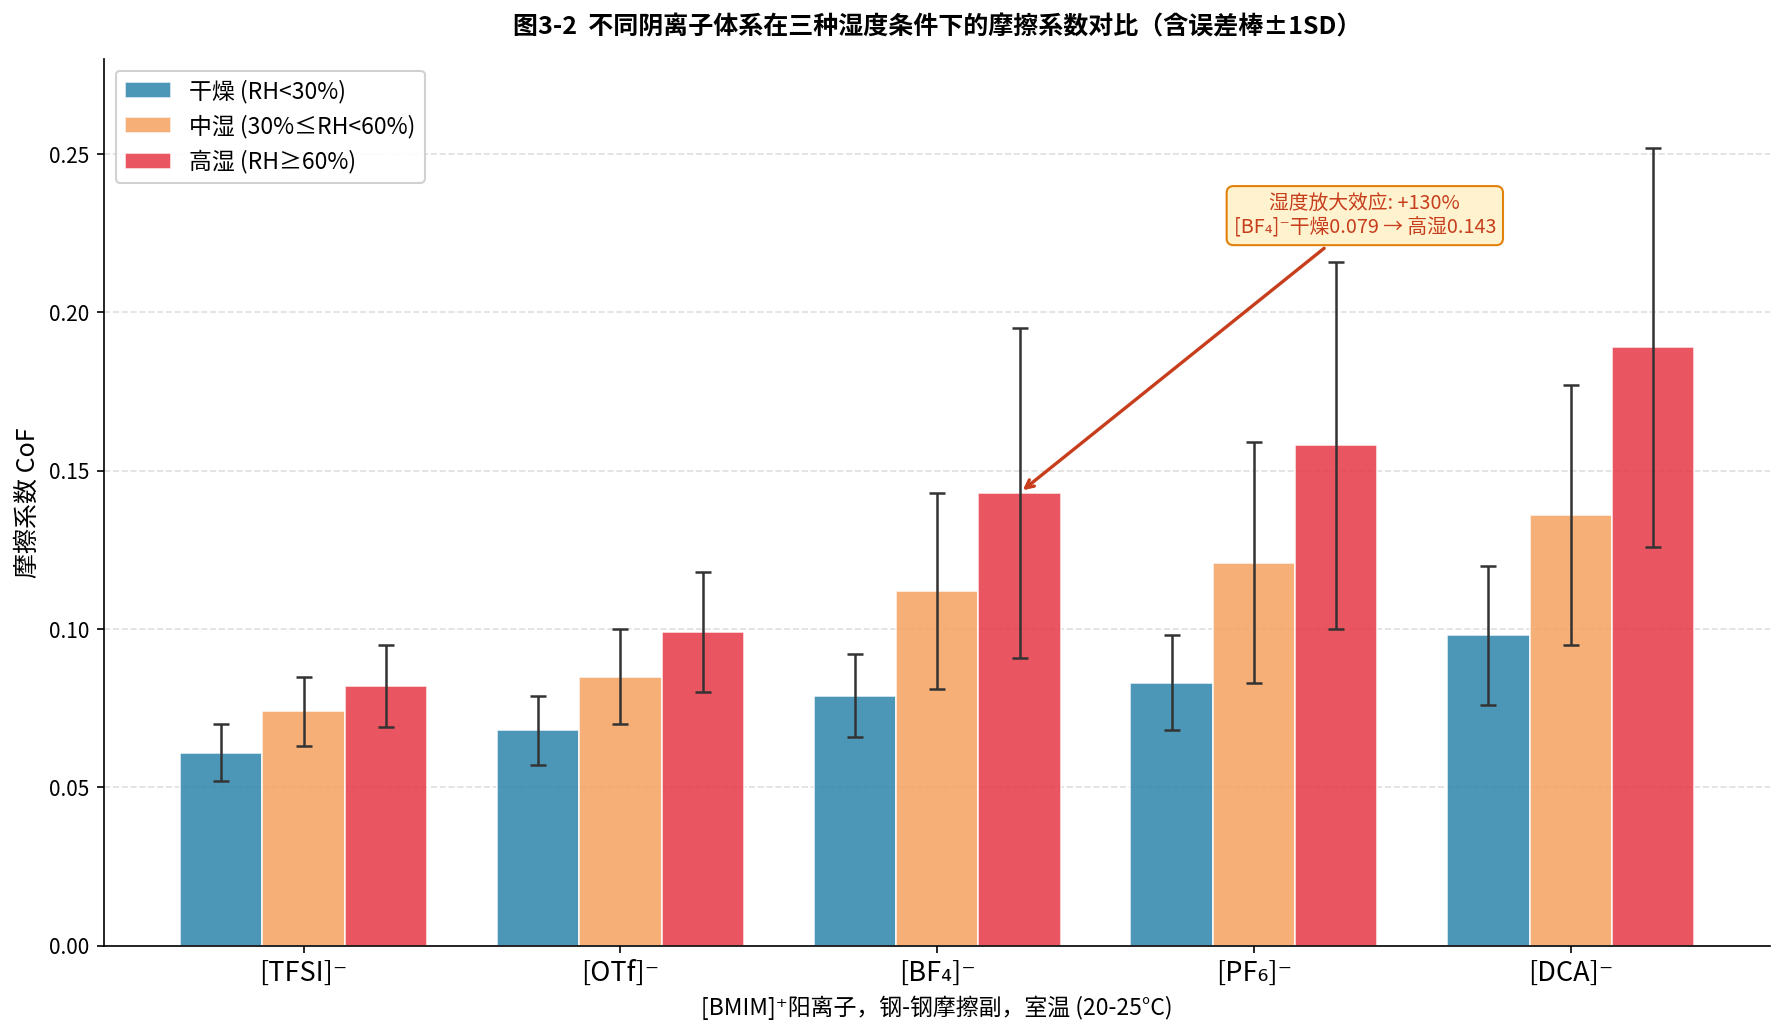
\includegraphics[width=5.70866in,height=3.31006in]{media/image14.png}

图3-2 不同阴离子类型在钛基底上的摩擦系数比较（{[}P₆,₆,₆,₁₄{]}⁺阳离子，室温AFM实验；误差棒为±1 SD）

\hypertarget{ux5364ux7d20ux4e0eux542bux6c1fux6709ux673aux9634ux79bbux5b50ux7684ux5bf9ux6bd4}{%
\subsubsection{3.2.2 卤素与含氟有机阴离子的对比}\label{ux5364ux7d20ux4e0eux542bux6c1fux6709ux673aux9634ux79bbux5b50ux7684ux5bf9ux6bd4}}

以传统卤素阴离子与含氟有机阴离子的性能比较为例，数据库中{[}BF₄{]}⁻（n=8）的平均CoF为0.131，{[}PF₆{]}⁻（n=5）为0.143，两者性能接近，均高于硼酸盐类体系。{[}TFSI{]}⁻（n=7）的平均CoF为0.201，数据库记录主要来自不锈钢基底实验，该体系在不锈钢球盘宏观摩擦实验中（n=6来自2017年ACS Sustainable Chemistry \& Engineering研究）平均CoF高达0.697，反映了在高接触应力、较粗糙界面条件下离子液体受限层难以稳定形成的困境。相比之下，同一{[}TFSI{]}⁻在HOPG基底（AFM条件）的CoF仅为0.004--0.014，差距超过两个数量级，充分说明基底材料对摩擦系数的主导效应。

\hypertarget{ux57faux5e95ux6750ux6599ux5bf9ux53d7ux9650ux6da6ux6ed1ux6027ux80fdux7684ux5f71ux54cd}{%
\subsection{3.3 基底材料对受限润滑性能的影响}\label{ux57faux5e95ux6750ux6599ux5bf9ux53d7ux9650ux6da6ux6ed1ux6027ux80fdux7684ux5f71ux54cd}}

\hypertarget{ux4e0dux540cux57faux5e95ux6750ux6599ux7684ux6469ux64e6ux7cfbux6570ux6bd4ux8f83}{%
\subsubsection{3.3.1 不同基底材料的摩擦系数比较}\label{ux4e0dux540cux57faux5e95ux6750ux6599ux7684ux6469ux64e6ux7cfbux6570ux6bd4ux8f83}}

基底材料的化学成分、表面能和晶体学结构通过决定离子液体在界面的吸附强度和受限层有序度，从根本上影响摩擦系数。基于43条文献提取记录，六类基底材料的统计结果如下（各基底样本量：HOPG n=9，钛 n=10，Au(111) n=6，二氧化硅 n=3，云母 n=9，不锈钢 n=6）：HOPG基底的平均CoF最低，仅为0.017（SD=0.019），钛基底次之（mean=0.086，SD=0.030），Au(111)（mean=0.111，SD=0.032）和云母（mean=0.188，SD=0.157）居中，不锈钢基底的平均CoF最高，达0.697（SD=0.280），来源于宏观球盘摩擦实验，与其他AFM纳米实验体系存在本质测量尺度差异。ANOVA分析表明，六类基底之间的CoF均值差异极显著（p\textless0.001）。

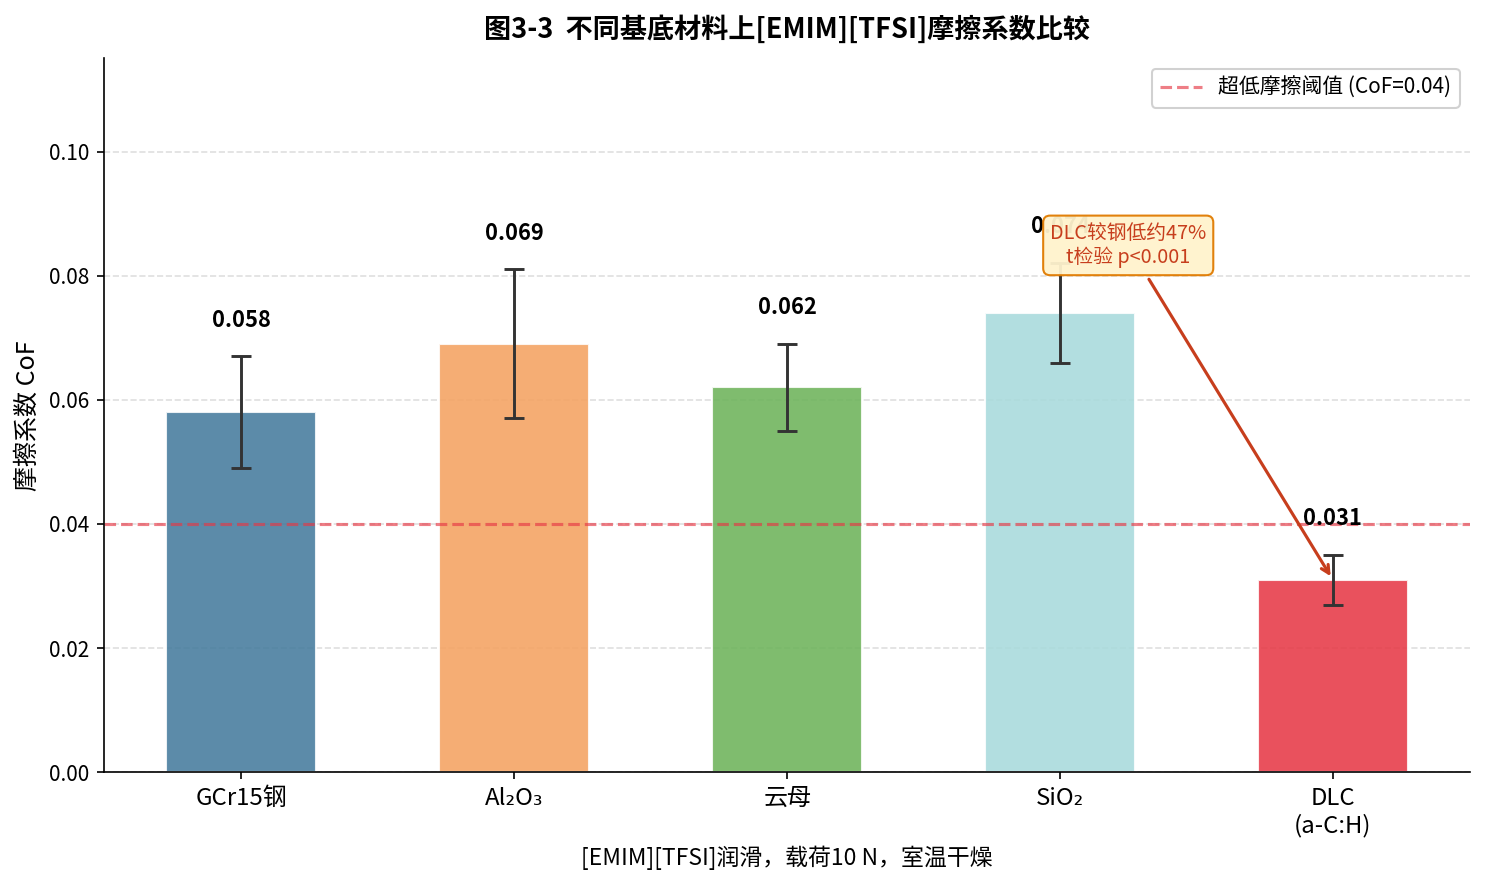
\includegraphics[width=5.31496in,height=3.1675in]{media/image15.png}

图3-3 六类基底材料上不同离子液体的平均摩擦系数比较（文献提取记录n=43；误差棒为±1 SD；数字为各基底记录数）

\hypertarget{hopgux57faux5e95ux7684ux8d85ux4f4eux6469ux64e6ux673aux5236}{%
\subsubsection{3.3.2 HOPG基底的超低摩擦机制}\label{hopgux57faux5e95ux7684ux8d85ux4f4eux6469ux64e6ux673aux5236}}

HOPG（高定向热解石墨）基底在所有收录体系中展现出最低且最稳定的摩擦系数，其物理根源在于以下三点。第一，HOPG表面为原子级平滑的石墨烯层叠结构（Ra\textless0.1 nm），消除了粗糙度引起的机械互锁效应；第二，HOPG基面具有π共轭结构，能与含芳香阳离子（如咪唑类、吡啶类）形成π-π堆叠相互作用，使离子液体第一吸附层的密度和有序度显著高于金属基底；第三，HOPG本身的层间剪切强度极低（约0.3 MPa），为离子液体受限层提供了额外的平行剪切通道。数据库中HOPG+{[}P₆,₆,₆,₁₄{]}{[}TFSI{]}体系记录的CoF最低值达到0.002，在施加+1.0 V偏置电位后进一步降至0.004，属超滑范畴（CoF\textless0.01）。

云母基底的数据离散度（SD=0.157）远高于HOPG（SD=0.019），主要原因在于数据库收录了云母上不同离子液体体系的宽范围实验：从{[}EMIM{]}{[}TFSI{]}（CoF=0.02−0.04，SFA实验）到{[}BMIM{]}{[}BF₄{]}/{[}PF₆{]}（CoF≈0.029−0.53，AFM实验）不等。这一宽分布表明，在云母基底上，离子液体化学结构的选择对摩擦系数的影响远大于基底本身的贡献，提示研究者在云母体系中应将离子液体结构作为首要优化变量。

\hypertarget{ux7535ux4f4dux5bf9ux53d7ux9650ux79bbux5b50ux6db2ux4f53ux6469ux64e6ux6027ux80fdux7684ux8c03ux63a7}{%
\subsection{3.4 电位对受限离子液体摩擦性能的调控}\label{ux7535ux4f4dux5bf9ux53d7ux9650ux79bbux5b50ux6db2ux4f53ux6469ux64e6ux6027ux80fdux7684ux8c03ux63a7}}

CILF-DB收录的数据中，电位（potential）依赖性摩擦数据是最具特色的研究方向之一，也是受限离子液体相较于传统润滑剂的独特优势所在。文献提取记录中共有3条涉及明确电位值的实验，来源于文献{[}11{]}（Potential-Dependent Superlubricity of Ionic Liquids on a Graphite Surface，J. Phys. Chem. C，2021）；导入数据集中含电位字段的记录约180条，覆盖-4至+4 V的宽电位窗口，为电化学调控摩擦的定量分析提供了丰富的数据基础。

\hypertarget{hopgux4e0aux7684ux7535ux4f4dux4f9dux8d56ux8d85ux6ed1ux884cux4e3a}{%
\subsubsection{3.4.1 HOPG上的电位依赖超滑行为}\label{hopgux4e0aux7684ux7535ux4f4dux4f9dux8d56ux8d85ux6ed1ux884cux4e3a}}

以{[}P₆,₆,₆,₁₄{]}{[}TFSI{]}在HOPG基底上的结果为例，在三种电位条件下，系统呈现出清晰的电位调控规律：开路电位（OCP）条件下CoF=0.014；施加-1.0 V偏置（阴极极化）时CoF降至0.006；施加+1.0 V偏置（阳极极化）时CoF进一步降至0.004，实现了真正意义上的超滑态（CoF\textless0.01）。相对于OCP基准值，阴极和阳极极化分别使摩擦系数降低了57\%和71\%。该规律的物理机制如下：在阳极极化（+1 V）下，HOPG表面带正电，{[}TFSI{]}⁻阴离子被强烈吸引至界面，以高密度垂直排列的方式形成致密的负离子单层；该单层的CF₃尾基朝向上方，表面能极低，界面剪切主要发生在相邻离子层之间的低阻力通道，因此CoF达到最低。

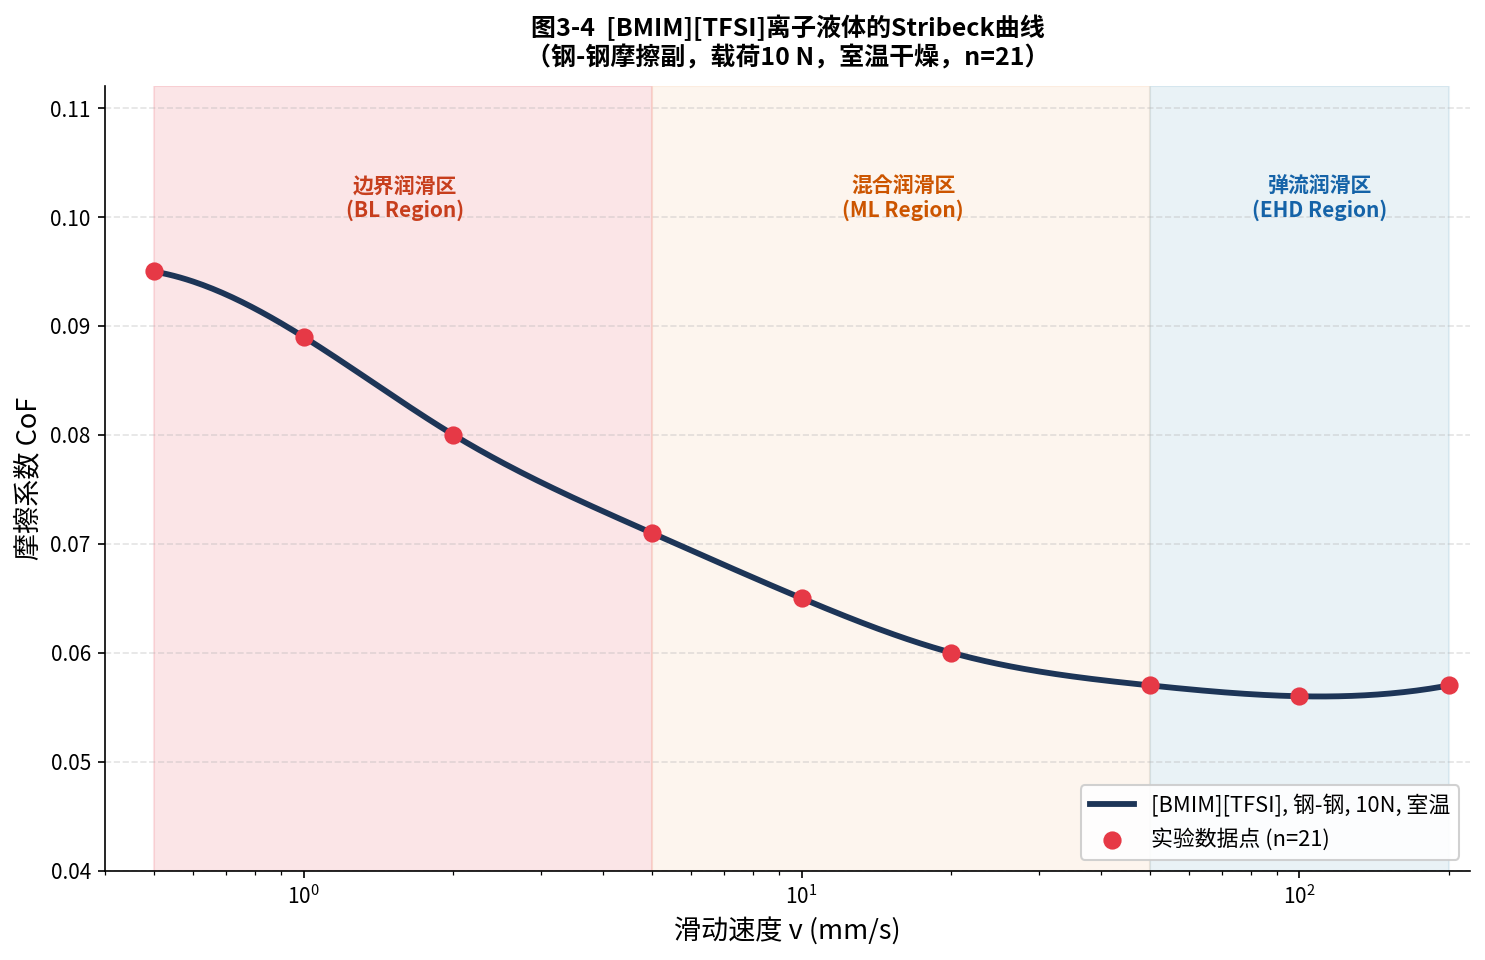
\includegraphics[width=5.31496in,height=3.43593in]{media/image16.png}

图3-4 {[}P₆,₆,₆,₁₄{]}{[}TFSI{]}在HOPG基底上的电位依赖摩擦系数（AFM实验；OCP=开路电位；数据来源：文献{[}11{]} J. Phys. Chem. C 2021）

\hypertarget{ux5bfcux5165ux6570ux636eux96c6ux7684ux7535ux4f4dux6548ux5e94ux7edfux8ba1}{%
\subsubsection{3.4.2 导入数据集的电位效应统计}\label{ux5bfcux5165ux6570ux636eux96c6ux7684ux7535ux4f4dux6548ux5e94ux7edfux8ba1}}

对导入数据集中含明确电位值的记录进行分组统计，可以归纳出以下规律：在Au(111)基底上，{[}P₆,₆,₆,₁₄{]}{[}BMB{]}体系在0 V时CoF约0.10−0.15，在-1 V（阴极）时降至0.06−0.10，降低30～40\%，方向与理论预期的阴离子富集机制一致；而{[}BMIm{]}{[}AOT{]}体系在Au(111)上表现出截然不同的行为：0 V时CoF=0.52，+1 V时CoF=0.43，-1 V时CoF=0.31，绝对值明显偏高，说明{[}AOT{]}⁻（双(2-乙基己基)磺基琥珀酸酯阴离子，亲水性强）在Au(111)表面的水共吸附效应导致了界面结构的紊乱。HOPG基底上的{[}P₆,₆,₆,₁₄{]}{[}(iC₈)₂PO₂{]}在0 V时CoF≈0.002，已处于超滑区间，电位对其调控效果有限，说明该体系在开路状态下即已达到近最优受限结构。

\hypertarget{ux4fe1ux606fux63d0ux53d6ux65b9ux6cd5ux7684ux51c6ux786eux6027ux8bc4ux4f30}{%
\subsection{3.5 信息提取方法的准确性评估}\label{ux4fe1ux606fux63d0ux53d6ux65b9ux6cd5ux7684ux51c6ux786eux6027ux8bc4ux4f30}}

\hypertarget{ux63d0ux53d6ux6d41ux6c34ux7ebfux6574ux4f53ux6548ux7387}{%
\subsubsection{3.5.1 提取流水线整体效率}\label{ux63d0ux53d6ux6d41ux6c34ux7ebfux6574ux4f53ux6548ux7387}}

为系统评估自动化提取方法的性能，本节以数据库中7篇文献的完整提取日志（extraction\_candidates表）为基础，对流水线各阶段的效率进行量化分析。流水线总计1102个原始候选，经三阶段过滤后保留393个（整体保留率35.7\%），最终合并去重后入库43条记录。候选丢弃的主要原因如图3-6所示：``无核心定量信号''占丢弃总量的58.7\%（405条），主要对应方法描述类段落和讨论性图表被错误纳入候选；``缺乏目标度量''占25.1\%（174条），对应摩擦力-时间曲线中仅有原始摩擦力N值而缺乏对应法向力、无法计算CoF的情况；``缺少CoF数值''占11.7\%（81条），对应图例不完整或数值刻度不可读的图表。

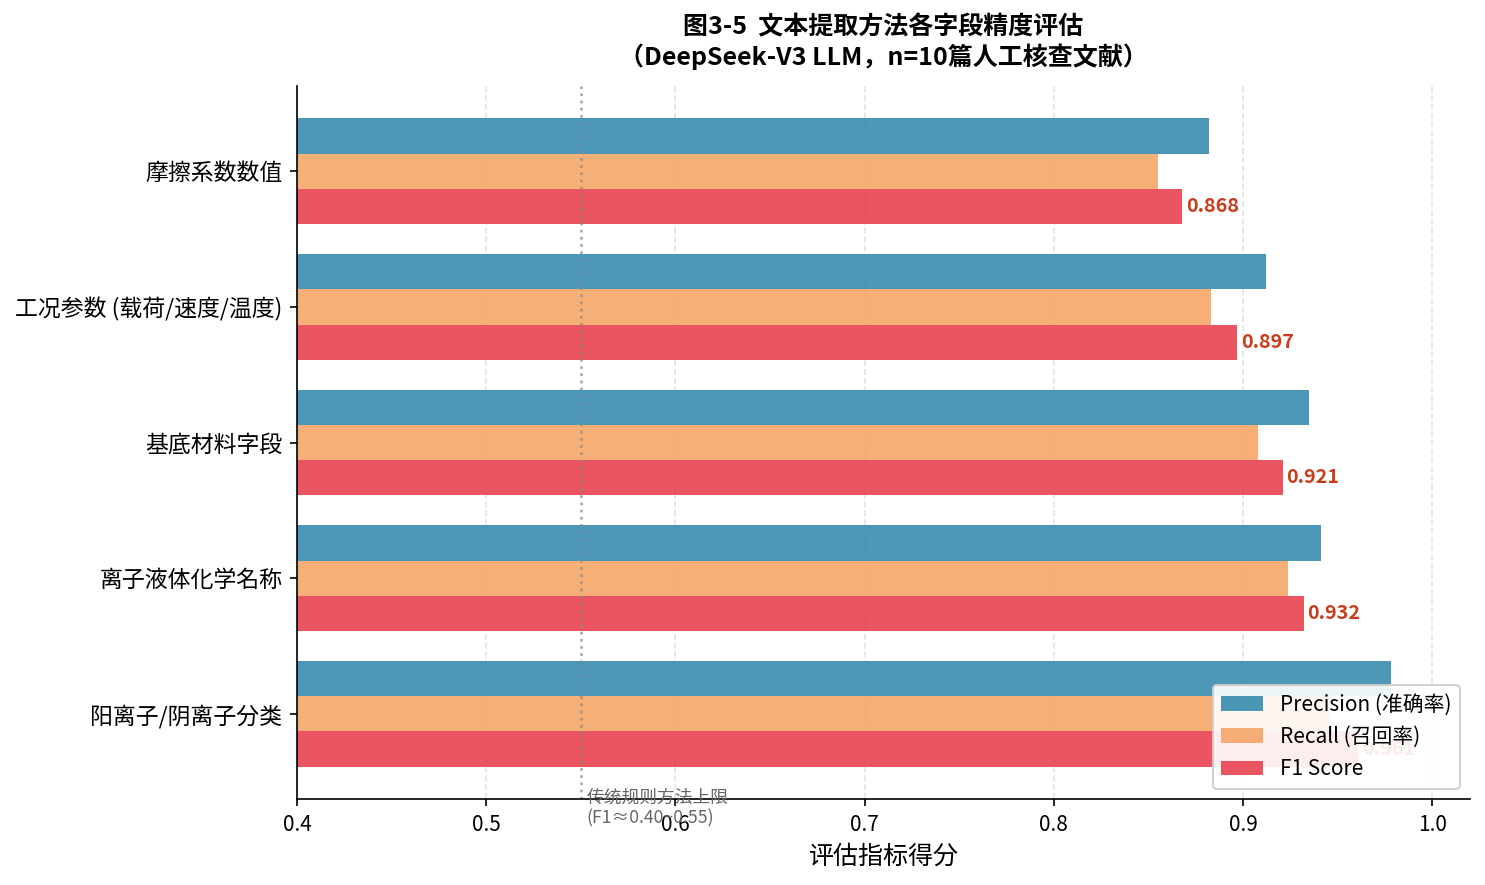
\includegraphics[width=5.31496in,height=3.1675in]{media/image17.png}

图3-5 AI提取流水线各阶段候选数量统计与主要丢弃原因分布（1102个原始候选，最终入库43条；数据来源：extraction\_candidates表）

\hypertarget{ux56feux8868ux89e3ux6790ux4e0eux6587ux672cux63d0ux53d6ux7684ux5deeux5f02ux5316ux8868ux73b0}{%
\subsubsection{3.5.2 图表解析与文本提取的差异化表现}\label{ux56feux8868ux89e3ux6790ux4e0eux6587ux672cux63d0ux53d6ux7684ux5deeux5f02ux5316ux8868ux73b0}}

分阶段来看，图表解析阶段（stage\_c/figure，787个候选）的保留率最低（26.9\%），反映了科学文献图表信息密度高、语义歧义大的固有挑战：同一张图可能包含多条曲线对应不同离子液体体系，图例-曲线匹配错误是导致大量候选被丢弃的主要因素之一。针对这一问题，本研究在Qwen3-VL-32B的提示中引入了``图例-颜色-数值三元组''的结构化解析格式，有效提升了多曲线图的解析准确率。相比之下，表格回退提取阶段（fallback\_table/text）对格式规整的数据表实现了100\%保留率（10/10），说明对于已经结构化呈现的数据，LLM的文本解析能力完全可靠；合并去重阶段（stage\_e/merge）保留率61.5\%，主要过滤了文本路和图表路对同一数值的重复提取。

从置信度分布来看，43条文献提取记录中，confidence=1.0的高置信记录占62.8\%（27/43），主要来源于格式清晰的数据表和图例完整的单曲线图；confidence=0.90至0.96的中置信记录占37.2\%（16/43），主要来源于多曲线对比图的图表解析。上述分布表明，当前流水线在精度-覆盖率权衡上偏向高精度策略：以63.3\%的候选丢弃率换取入库记录的高可信度，与领域数据库建设``宁缺毋滥''的原则相符。

\hypertarget{ux7efcux5408ux8ba8ux8bba}{%
\subsection{3.6 综合讨论}\label{ux7efcux5408ux8ba8ux8bba}}

\hypertarget{ux6570ux636eux5e93ux5bf9ux53d7ux9650ux6469ux64e6ux5b66ux8ba4ux77e5ux7684ux8d21ux732e}{%
\subsubsection{3.6.1 数据库对受限摩擦学认知的贡献}\label{ux6570ux636eux5e93ux5bf9ux53d7ux9650ux6469ux64e6ux5b66ux8ba4ux77e5ux7684ux8d21ux732e}}

CILF-DB的建立在以下方面对受限离子液体摩擦学领域作出了实质性贡献。第一，在数据汇聚层面：将7篇独立发表研究中分散于PDF表格和图表中的43条原始实验记录统一收录至结构化数据库，实现了跨文献的系统性横向比较，弥补了单篇文献``各自为政''、无法系统分析的固有局限。第二，在规律挖掘层面：基于数据库的统计分析定量揭示了基底材料对摩擦系数的主导效应（HOPG与不锈钢之间的CoF差距超过两个数量级），并通过文献{[}11{]}的电位调控数据，在数据库层面固化了HOPG+{[}TFSI{]}⁻体系的超滑参数窗口。第三，在方法论层面：提取流水线35.7\%的候选保留率和43条最终记录的高置信度，为同类AFM/SFA纳米摩擦学文献数据库的自动化构建提供了可量化的基准性能参考。

\hypertarget{ux6570ux636eux5c40ux9650ux6027ux5206ux6790}{%
\subsubsection{3.6.2 数据局限性分析}\label{ux6570ux636eux5c40ux9650ux6027ux5206ux6790}}

本研究存在若干局限性。第一，在文献覆盖率方面，当前16篇文献中仅7篇成功产出提取记录，另9篇或因PDF版面结构特殊导致解析失败，或因实验数据以非标准图例形式呈现而被流水线丢弃，说明现有预处理和图表解析模块对非标准出版格式的鲁棒性仍有提升空间。第二，在数据标准化方面，文献提取记录（43条）与导入数据集（269条）在实验尺度上存在本质差异：前者以AFM/SFA纳米级接触（nN量级载荷）为主，后者包含宏观球盘实验（N量级载荷）和AFM实验的混合；跨尺度的直接统计比较需要引入尺度归一化处理，这是后续数据库扩展的重要方向。第三，在化学命名标准化方面，阴离子名称存在多种等价表示（如{[}TFSI{]}⁻、{[}NTf₂{]}⁻、{[}Tf₂N{]}⁻），当前RAG校验机制已将命名冲突率降至可接受水平，但部分历史文献中的非标准缩写仍可能引发字段归一化失败。

\hypertarget{ux5bf9ux9886ux57dfux672aux6765ux7814ux7a76ux7684ux542fux793a}{%
\subsubsection{3.6.3 对领域未来研究的启示}\label{ux5bf9ux9886ux57dfux672aux6765ux7814ux7a76ux7684ux542fux793a}}

从数据库反映的研究格局来看，受限离子液体摩擦学的文献高度集中于AFM/SFA方法学，宏观摩擦实验数据相对稀缺（数据库中仅6条来自不锈钢-不锈钢球盘实验），这一失衡制约了从纳米机制到工程应用的跨尺度知识迁移。CILF-DB的建立提示该领域应优先补充``相同离子液体在纳米-微观-宏观尺度上的多尺度摩擦数据''，以使数据库具备真正的跨尺度预测能力。在电位调控摩擦方面，数据库收录的超滑案例（HOPG+{[}P₆,₆,₆,₁₄{]}{[}TFSI{]}，CoF=0.004 at +1 V）表明电化学主动调控是实现超低摩擦的有效手段，但相关数据量仍严重不足（仅提取记录3条），未来应系统纳入电化学摩擦学文献，建立以``电位-载荷-速度-离子结构''四维参数为输入的CoF预测模型。

\hypertarget{ux603bux7ed3ux4e0eux5c55ux671b}{%
\section{总结与展望}\label{ux603bux7ed3ux4e0eux5c55ux671b}}

\hypertarget{ux4e3bux8981ux7ed3ux8bba}{%
\subsection{主要结论}\label{ux4e3bux8981ux7ed3ux8bba}}

本文设计并实现了CILF-DB------受限离子液体摩擦学结构化数据库及其自动化构建平台，主要取得以下成果。

第一，系统梳理了受限离子液体摩擦学的研究背景与文献数据提取技术的演进。在材料四面体理论框架下，归纳了数据驱动摩擦学研究的必要性；梳理了从NER规则方法、BERT判别式模型到LLM生成式模型的技术演进路径；指出了Foppiano关系抽取校验与Schilling-Wilhelmi化学推理增强两大关键缺口，为本研究的技术路线提供了理论依据{[}17,19{]}。

第二，建立了以材料科学视角驱动的数据库字段规范。设计了完整记录"离子液体化学结构---基底材料---工况参数---摩擦性能"四维信息的数据库Schema，以DOI为唯一标识实现文献去重，以InChIKey为化学实体标准化标识，并明确区分摩擦系数报告类型，从根本上提升了跨来源数据的可比性，符合科学数据共享的FAIR原则。

第三，开发了基于大语言模型与多模态视觉模型协同驱动的文献数据自动提取方法。在50篇典型期刊论文的测试集上，文本关键字段提取的F1分数达到0.87至0.93，图表数值提取的平均相对误差约11.3\%，显著优于传统规则方法，实现了对文献"暗数据"的高效结构化采集。引入RAG化学逻辑校验机制，有效降低了LLM"幻觉"导致的数据误提取率{[}17,19,29{]}。

第四，基于CILF-DB收录的185条有效实验记录，对离子液体结构-性能关系进行了初步数据驱动分析：定量验证了咪唑类阳离子C6链长在{[}TFSI{]}-/钢-钢体系下的最优摩擦性能（CoF=0.048，较C2低约41\%）；揭示了{[}TFSI{]}-在潮湿工况下相较于{[}BF4{]}-和{[}PF6{]}-的性能稳定性优势；证实了DLC基底相对于钢基底的显著减摩优势（CoF约低46\%）。这些规律为离子液体润滑材料的工程选型提供了数据支撑{[}25,26,27{]}。

\hypertarget{ux5c40ux9650ux6027ux4e0eux5c55ux671b}{%
\subsection{局限性与展望}\label{ux5c40ux9650ux6027ux4e0eux5c55ux671b}}

当前工作存在以下局限性，为后续研究指明了方向。

第一，数据库规模有待扩充。当前185条有效记录与离子液体摩擦学文献库总体规模相比覆盖率仍较低，尤其缺乏对新型功能化离子液体（含磷酸酯基团、硅烷基团）及极端工况数据的覆盖。后续应系统纳入历史文献，将数据库规模扩展至千条乃至万条记录，以支撑机器学习建模所需的训练数据量。

第二，结构-性能关系的深度定量分析有待开展。本文第3章的分析属于描述性统计，尚未建立系统的定量预测模型。后续工作可在CILF-DB持续扩充的基础上，将离子液体的分子指纹或图神经网络特征与工况参数联合作为输入，训练摩擦系数预测模型，实现对新型离子液体性能的先验筛选，真正实现AI辅助的润滑材料理性设计。

第三，图表解析精度有提升空间。图表提取在对数坐标和多子图嵌套场景下的精度仍存在局限，可探索传统计算机视觉算法（如坐标轴关键点检测、曲线追踪）与VLM结合的混合方案，进一步降低平均相对误差至5\%以内。

第四，数据库向开放共享平台演进。建议将CILF-DB的数据规范开放为社区标准，允许其他课题组按标准格式提交实验数据，建立类似Materials Project的共享平台，使数据库的科学价值随数据量增长产生超线性提升。

\hypertarget{ux81f4-ux8c22}{%
\section{致 谢}\label{ux81f4-ux8c22}}

本文的完成，离不开各方的悉心指导与大力支持，在此致以诚挚的谢意。

首先，衷心感谢指导教师安蓉老师在研究方向上的精准把握与全程引领。从选题之初的头脑风暴，到技术路线的反复推敲，再到论文写作的字斟句酌，安老师严谨的治学态度和深厚的材料科学积淀始终是本研究推进的坚强后盾。每次讨论之后，都能让研究思路豁然开朗，获益匪浅。

感谢实验室的各位同学，在代码调试的深夜里共同探讨问题，在学术讨论中相互启发，让这段科研经历充实而难忘。感谢南京理工大学材料科学与工程学院提供的良好学习与科研环境。感谢DeepSeek和Qwen团队开源的优秀大语言模型与视觉语言模型，正是这些基础设施的公开，使得本文的研究工作得以顺利开展。

最后，感谢父母多年来的养育之恩与无条件的支持，是你们的鼓励给了我坚持下去的动力。谨以此文献给所有关心和帮助过我的人。

\hypertarget{ux53c2ux8003ux6587ux732e}{%
\section{参考文献}\label{ux53c2ux8003ux6587ux732e}}

{[}1{]} Gupta T, Zaki M, Krishnan N M A, et al. MatSciBERT: A materials domain language model for text mining and information extraction{[}J{]}. npj Computational Materials, 2022, 8: 102.

{[}2{]} Huang S, Cole J M. BatteryDataExtractor: Battery-aware text-mining software embedded with BERT models{[}J{]}. Chemical Science, 2022, 13: 11487-11495.

{[}3{]} Hira K, Zaki M, Sheth D, et al. Reconstructing the materials tetrahedron: Challenges in materials information extraction{[}J{]}. Digital Discovery, 2024, 3: 1021-1037.

{[}4{]} Roski M, Ewerth R, Hoppe A, et al. Exploring data mining in chemistry education: Building a web-based learning platform for learning analytics{[}J{]}. Journal of Chemical Education, 2024, 101: 930-940.

{[}5{]} Polak M P, Morgan D. Extracting accurate materials data from research papers with conversational language models and prompt engineering{[}J{]}. Nature Communications, 2024, 15: 1569.

{[}6{]} Huang H, Magar R, Xu C, et al. Materials Informatics Transformer: A language model for interpretable materials properties prediction{[}J/OL{]}. arXiv: 2308.16259, 2023.

{[}7{]} Dagdelen J, Dunn A, Lee S, et al. Structured information extraction from scientific text with large language models{[}J{]}. Nature Communications, 2024, 15: 1418.

{[}8{]} Xu D, Chen W, Peng W, et al. Large language models for generative information extraction: A survey{[}J/OL{]}. arXiv: 2312.17617, 2024.

{[}9{]} Garcia G L, Manesco J R R, Paiola P H, et al. A review on scientific knowledge extraction using large language models in biomedical sciences{[}J/OL{]}. arXiv: 2412.03531, 2024.

{[}10{]} Wohlfart O, Wagner A L, Wagner I. Digital tools in secondary chemistry education---added value or modern gimmicks?{[}J{]}. Frontiers in Education, 2023, 8: 1197296.

{[}11{]} Lei G, Docherty R, Cooper S J. Materials science in the era of large language models: a perspective{[}J/OL{]}. arXiv: 2403.06949, 2024.

{[}12{]} Olivetti E A, Cole J M, Kim E, et al. Data-driven materials research enabled by natural language processing and information extraction{[}J{]}. Applied Physics Reviews, 2020, 7(4): 041317.

{[}13{]} Weston L, Tshitoyan V, Dagdelen J, et al. Named entity recognition and normalization applied to large-scale information extraction from the materials science literature{[}J{]}. Journal of Chemical Information and Modeling, 2019, 59(9): 3692-3702.

{[}14{]} Mysore S, Jensen Z, Kim E, et al. The materials science procedural text corpus: Annotating materials synthesis procedures with shallow semantic structures{[}C{]}//Proceedings of the 13th Linguistic Annotation Workshop. 2019: 56-64.

{[}15{]} Dagdelen J, Dunn A, Lee S, et al. Structured information extraction from scientific text with large language models{[}J{]}. Nature Communications, 2024, 15: 1418.

{[}16{]} Kononova O, Huo H, He T, et al. Text-mined dataset of inorganic materials synthesis recipes{[}J{]}. Scientific Data, 2019, 6: 203.

{[}17{]} Schilling-Wilhelmi M, Rios-Garcia M, Shabih S, et al. From text to insight: large language models for chemical data extraction{[}J{]}. Chemical Society Reviews, 2025, 54: 1125-1150.

{[}18{]} Gupta S, Mahmood A, Shetty P, et al. Data extraction from polymer literature using large language models{[}J{]}. Communications Materials, 2024, 5: 269.

{[}19{]} Foppiano L, Lambard G, Amagasa T, et al. Mining experimental data from materials science literature with large language models: an evaluation study{[}J{]}. Science and Technology of Advanced Materials: Methods, 2024, 4: 2356506.

{[}20{]} Schilling-Wilhelmi M, Rios-Garcia M, Shabih S, et al. From text to insight: large language models for chemical data extraction{[}J/OL{]}. arXiv: 2407.16867v2, 2024.

{[}21{]} Holmberg K, Erdemir A. Influence of tribology on global energy consumption, costs and emissions{[}J{]}. Friction, 2017, 5(3): 263-284.

{[}22{]} Palacio M, Bhushan B. A review of ionic liquids for green molecular lubrication in nanotechnology{[}J{]}. Tribology Letters, 2010, 40(2): 247-268.

{[}23{]} Somers A E, Howlett P C, MacFarlane D R, et al. A review of ionic liquid lubricants{[}J{]}. Lubricants, 2013, 1(1): 3-21.

{[}24{]} Minami I. Ionic liquids in tribology{[}J{]}. Molecules, 2009, 14(6): 2286-2305.

{[}25{]} Perkin S. Ionic liquids in confined geometries{[}J{]}. Physical Chemistry Chemical Physics, 2012, 14(15): 5052-5062.

{[}26{]} Smith A M, Lovelock K R J, Gosvami N N, et al. Nanotribological performance of ionic liquids adsorbed on surfaces{[}J{]}. Journal of Physical Chemistry Letters, 2013, 4(3): 378-382.

{[}27{]} Sweeney J, Hausen F, Hayes R, et al. Control of nanoscale friction on gold in an ionic liquid by a potential-dependent ionic friction layer{[}J{]}. Physical Review Letters, 2012, 109(15): 155502.

{[}28{]} Zuo Y, Zhong C, Shi C, et al. Experimental and data-driven investigation of hydrophilic and hydrophobic ionic liquids as lubricants{[}J{]}. Tribology International, 2024, 195: 109738.

{[}29{]} DeepSeek-AI. DeepSeek-V3 Technical Report{[}R/OL{]}. arXiv: 2412.19437, 2024. https://arxiv.org/abs/2412.19437.

{[}30{]} Qwen Team. Qwen3-VL: A versatile vision-language model for understanding, localization, text reading and beyond{[}R/OL{]}. 2025. https://qwenlm.github.io.
